\documentclass[a4paper,12pt]{article}

\usepackage[utf8]{inputenc}
\usepackage[ngerman]{babel}
\usepackage{lmodern}
\usepackage{aliascnt}
\usepackage{csquotes}
\usepackage[locale=US]{siunitx}
\usepackage{float}

\usepackage{float}
\floatstyle{ruled}
\newaliascnt{listing}{figure}
\newfloat{listing}{htbp}{lop}
\floatname{listing}{Listing}
\aliascntresetthe{listing}


\usepackage[margin=2.5cm]{geometry}
\usepackage{fontspec}
%\usepackage{courier}
\usepackage{listings}
\usepackage{caption}
\captionsetup{
    font=small,              % kleinere Schrift
    labelfont=bf,            % "Abbildung 1" fett
    textfont=it,             % Rest kursiv
    skip=0.7em               % Abstand zur Abbildung
}

\usepackage{amsmath}
\usepackage{amssymb}
\usepackage[colorlinks=true,
	    linkcolor=blue,
	    citecolor=blue,
	    urlcolor=blue]{hyperref}
\usepackage{booktabs}
\usepackage{graphicx}
\usepackage[most]{tcolorbox}
\usepackage{xcolor}
%\setmonofont{Andale Mono}
%\setmonofont{Inconsolata}
%\setmonofont{JetBrains Mono}
%\setmonofont{Source Code Pro}

\definecolor{myblue}{RGB}{3, 77, 128}

\title{Blinkende LED – ein Blick unter die Haube}
\author{}
\date{}


\newcommand{\monoscale}{Scale=0.91}

\setmonofont{Fira Mono}[\monoscale]
\newfontfamily\firamono{Fira Mono}[\monoscale]

\lstset{
    basicstyle=\firamono\small,
    columns=flexible,
    breaklines=true,
}

\usepackage{tikz}
\usetikzlibrary{
    shapes.geometric,
    arrows.meta,
    positioning,
    decorations.pathreplacing
}


\tikzstyle{box} = [
    rectangle, draw,
    rounded corners,
    minimum width=5cm,
    minimum height=1.2cm,
    text centered,
    align=center,
    draw=black,
    fill=gray!10
]
\tikzstyle{jump} = [
    diamond,
    aspect=2,
    draw,
    minimum width=5.5cm,
    text centered,
    align=center,
    fill=myblue!10,
    inner sep=1mm
]
\tikzstyle{arrow} = [
    thick,
    ->,
    >=stealth
]

\providecommand*{\listingautorefname}{Listing}

\begin{document}

\maketitle

\section{Ziel dieses Projektabschnitts}

Viele arbeiten beim Programmieren eines Mikrocontrollers mit der Arduino-IDE.
Dort reicht es, den C/C++-Code einzutippen und auf einen Button zu klicken –
der Code wird kompiliert und direkt auf den Mikrocontroller übertragen
(geflasht). Einfach und bequem.

In diesem Projektabschnitt wollen wir verstehen, was genau passiert, wenn
man auf diesen Knopf drückt. Wir lassen die Arduino-IDE beiseite und schreiben
den Maschinencode direkt selbst. Das heißt: Wir erstellen die Programmdatei per
Hand – wie echte Hacker oder Ingenieure, die wissen wollen, was wirklich läuft.

Wir beschäftigen uns dabei zwar noch nicht mit Assembler – das kommt später.
Stattdessen schreiben wir den Maschinencode direkt, also Byte für Byte. Das ist
etwas, das man als Techniker oder Ingenieur einmal im Leben gemacht haben
sollte – schon allein, um zu verstehen, was eine höhere Programmiersprache
überhaupt leistet.  Die eigentliche Herausforderung ist dabei nicht der
Maschinencode selbst, sondern der Umgang mit dem Terminal:
\begin{itemize}
    \item
	Wie schreibt man eine Datei im Editor \texttt{nano}?
    \item
	Wie organisiert man sich Verzeichnisse?
    \item
	Wie navigiert man im Terminal und lässt sich Dateien anzeigen?
    \item
	Und wie überträgt man schließlich mit \texttt{avrdude} den
	Maschinencode auf den Mikrocontroller?
\end{itemize}

\noindent
All das sind wichtige Grundlagen – und nach diesem Abschnitt könnt ihr von euch
behaupten: Ich habe ein Mikrocontrollerprogramm direkt in Maschinencode
geschrieben und selbst geflasht.

Aber das ist noch nicht alles. Das praktische Ziel wird es sein, eine LED
blinken zu lassen. Genauer gesagt soll sie abwechselnd 250\,ns an und 250\,ns
aus sein. Mit dem bloßen Auge kann man das nicht mehr sehen – wir werden das
deshalb mit dem Oszilloskop nachmessen.  Die Periodendauer beträgt dabei
\[
T = 250\,\text{ns} + 250\,\text{ns} = 500\,\text{ns},
\]
was einer Frequenz von
\[
f = \frac{1}{T} = \frac{1}{500\,\text{ns}} = 2\,\text{MHz}
\]
entspricht.

Bei unserem ersten Experiment werden wir zwar sehen, dass wir ein Signal
erzeugen, bei dem die LED an- und ausgeschaltet wird, es wird aber nicht
symmetrisch sein. Das ist aber nicht schlimm – wir werden bei der Gelegenheit
eben doch etwas mehr darüber lernen, wie der Maschinencode ausgeführt wird.

Und weil das Schreiben von Maschinencode zwar nicht schwer, aber mühsam ist,
wechseln wir anschließend doch auf eine höhere Sprache – aber noch nicht C/C++,
sondern zunächst auf Assembler. Mit einem Assembler (\texttt{avr-as}) kann man
den Code in Maschinencode übersetzen. Im Vergleich zu C/C++ sieht man hier
sofort, dass man eigentlich exakt dasselbe wie im Maschinencode macht, nur
komfortabler.\footnote{Analog ist aber auch C/C++ nur eine komfortable und
portable Weise, um Assemblercode kompakt auszudrücken.}

\newpage
\section{Einfaches Programm zur Ansteuerung einer LED}

Um eine LED schnell blinken zu lassen, benötigen wir nur vier Maschinenbefehle: 

\begin{itemize}
    \item
	einen, um den gewünschten Pin des Mikroprozessors als Ausgang zu
	konfigurieren,
    \item
	einen, um diesen Pin auf \texttt{HIGH} zu setzen (also Spannung
	anzulegen),
    \item
	einen, um ihn auf \texttt{LOW} zu setzen (also die Spannung wieder
	wegzunehmen),
    \item
	und einen sogenannten \emph{Sprungbefehl}, mit dem die
	Programmausführung an einer anderen Stelle fortgesetzt werden kann.
\end{itemize}

\noindent
Jeder dieser Befehle besteht aus zwei Bytes und kann daher mit vier
Hexadezimalziffern dargestellt werden. Die Befehle werden nacheinander
(sequenziell) abgearbeitet – wie im folgenden Ablaufdiagramm dargestellt:


\begin{center}
\begin{tikzpicture}[scale=0.8, every node/.style={transform shape}, node distance=0.7cm and 0.8cm]

\node (step1) [box]
    {Hex: \texttt{52 9a}\\\small Pin 2 als Ausgang benutzen};
\node (step2) [box, below=of step1]
    {Hex: \texttt{5a 9a}\\\small Pin 2 auf \texttt{HIGH} setzen};
\node (step3) [box, below=of step2]
    {Hex: \texttt{5a 98}\\\small Pin 2 auf \texttt{LOW} setzen};
\node (step4) [jump, below=of step3]
    {Hex: \texttt{fd cf}\\\small 2 Befehle zurück};

\draw [arrow] (step1) -- (step2);
\draw [arrow] (step2) -- (step3);
\draw [arrow] (step3) -- (step4);

% Rücksprungpfeil
\draw [arrow] (step4.east) -- ++(1.5,0) node[right] {} 
              |- (step2.east);

\end{tikzpicture}
\end{center}

\noindent
Schreibt man die Hexadezimalwerte der Befehle nacheinander auf, ergibt sich
unser erstes vollständiges Programm in Maschinencode:
\begin{center}
    \texttt{52 9a 5a 9a 5a 98 fd cf}
\end{center}
Jede Hex-Ziffer steht dabei für genau vier Bits. Die vollständige Bitbedeutung
kann man in \autoref{tab:bitmuster} nachschlagen.  In binärer Darstellung sieht
unser Programm dann so aus:
\begin{center}
    \texttt{01010010 10011010 01011010 10011010 01011010 10011000 11111101 11001111}
\end{center}

\begin{table}[ht]
    \centering
    \caption{Darstellung aller 4-Bit-Zahlen in dezimaler, hexadezimaler und binärer Form}
    \label{tab:bitmuster}
    \begin{tabular}{c c c}
        \textbf{Dezimal} & \textbf{Hexadezimal} & \textbf{Binär} \\
        \hline
         0 & 0  & 0000 \\
         1 & 1  & 0001 \\
         2 & 2  & 0010 \\
         3 & 3  & 0011 \\
         4 & 4  & 0100 \\
         5 & 5  & 0101 \\
         6 & 6  & 0110 \\
         7 & 7  & 0111 \\
         8 & 8  & 1000 \\
         9 & 9  & 1001 \\
        10 & A  & 1010 \\
        11 & B  & 1011 \\
        12 & C  & 1100 \\
        13 & D  & 1101 \\
        14 & E  & 1110 \\
        15 & F  & 1111 \\
    \end{tabular}
\end{table}

\noindent
Das Programm ist nun vollständig entworfen. Es fehlt nur noch ein letzter
Schritt: Es muss in den Programmspeicher des Mikroprozessors geschrieben werden
– also in den sogenannten \emph{Flash}-Speicher.

\noindent
Im nächsten Abschnitt wird erklärt, wie man den Maschinencode in
Hexadezimaldarstellung in eine Datei schreibt und mit dem Programm
\texttt{avrdude} in den Flash-Speicher des Mikroprozessors überträgt.

Was heute mit einem einzigen Befehl erledigt ist, war bei historischen
Computern und Mikroprozessoren der 1950er bis 1970er Jahre deutlich
aufwändiger:
Programme wurden oft bitweise geladen, indem für jedes einzelne Bit (binary
digit, also Binärziffer) ein Kippschalter umgelegt wurde.
\footnote{Das Eingeben von Programmen per Kippschalter war in den 1970er Jahren
ganz normal – vom Altair 8800 im Hobbykeller bis zu den legendären
Supercomputern von Seymour Cray, dem Pionier des Hochleistungsrechnens. Beim
Altair musste man den Bootloader Bit für Bit über das Frontpanel eintippen,
LEDs zeigten den aktuellen Speicherinhalt. Auch Cray setzte bei seinen frühen
Maschinen den ersten Code per Hand, bevor Magnetbandlaufwerke größere Programme
nachluden.}
Alternativ wurden Programme auf Lochkarten gestanzt und mechanisch eingelesen –
was im Prinzip ebenfalls nichts anderes bedeutete, als viele Bits in Folge
einzugeben, nur eben etwas bequemer.
Man kann sich diese alten Verfahren heute als Gedankenmodell gut vorstellen, um
besser zu verstehen, was das Programm \texttt{avrdude} im Hintergrund
eigentlich für uns erledigt.

\newpage

\section{
    Das Programm in den Mikroprozessor übertragen (den Mikroprozessor
    „flashen“)
}

\begin{figure}[ht]
\centering
\begin{tikzpicture}[
    node distance=0.7cm and .8cm,
    font=\sffamily,
    box/.style={
        draw,
        minimum width=4.8cm,
        minimum height=3cm,
        align=center,
        rounded corners,
        fill=gray!10
    }
]

% Speicherblöcke
\node[box] (flash) {
    \textbf{Flash-Speicher} \\
    \small 32 KB \\
    (0x0000 – 0x7FFF) \\
    \scriptsize enthält Programmcode \\
    \scriptsize (Maschinencode)
};

\node[box, right=of flash] (sram) {
    \textbf{SRAM} \\
    \small 2304 Bytes \\
    (0x0000 – 0x08FF) \\
    \scriptsize enthält Register, I/O-Register \\
    \scriptsize sowie Daten (Variablen, Stack)
};

\node[box, right=of sram] (eeprom) {
    \textbf{EEPROM} \\
    \small 1 KB \\
    (0x000 – 0x3FF) \\
    \scriptsize speichert Daten dauerhaft\\
    \scriptsize (z. B. Konfiguration)
};

\end{tikzpicture}
\caption{
    Speicheraufbau des ATmega328P: Der Flash enthält das Programm, der SRAM
    enthält Register, I/O-Bereiche und Daten. Der EEPROM speichert
    nicht-flüchtige Nutzdaten.
}
\label{fig:speicherarten}
\end{figure}

\noindent
Unser Mikroprozessor verfügt über drei verschiedene Arten von Speicher
(\autoref{fig:speicherarten}):

\begin{itemize}
    \item
	Einen Speicher für das Programm – den sogenannten \emph{Flash}. Dort
	bleiben die Daten auch erhalten, wenn man den Stecker zieht.
    \item
	Einen \emph{flüchtigen Speicher} (RAM), der während der
	Programmausführung zur Verfügung steht. Die Daten darin gehen verloren,
	sobald der Strom weg ist.
    \item
	Einen sogenannten \emph{EEPROM} (Electrically Erasable Programmable
	Read-Only Memory), in dem man dauerhaft kleine Datenmengen speichern
	kann – z.\,B. Konfigurationen oder Zustände, die auch nach dem
	Ausschalten erhalten bleiben sollen.
\end{itemize}

\noindent
Für uns ist zunächst nur der Flash-Speicher wichtig – in ihn muss unser
Programm übertragen werden.  Allen Speicherarten ist gemeinsam: Sie bestehen
aus Arrays von Speicherzellen.  In jeder Zelle kann genau ein Byte gespeichert
werden, also 8 Bits. Diese 8 Bits lassen sich kompakt durch zwei
Hexadezimalziffern darstellen. Die Speicherzellen sind durchnummeriert – diese
Nummer nennt man \emph{Adresse}.  Die erste Adresse hat immer den Wert 0.
Unser Ziel ist es, dass der Programmspeicher nach dem Flashen so aussieht:


\begin{center}
\begin{tikzpicture}
% Größe und Abstand
\def\cellsize{1cm}

% Zeichne 12 Zellen
\foreach \i in {0,...,11} {
    \draw (\i*\cellsize, 0) rectangle ++(\cellsize, \cellsize);
}

% Trage die Bytes in die ersten 8 Zellen ein
\node at (0.5*\cellsize, 0.5*\cellsize) {\ttfamily 52};
\node at (1.5*\cellsize, 0.5*\cellsize) {\ttfamily 9a};
\node at (2.5*\cellsize, 0.5*\cellsize) {\ttfamily 5a};
\node at (3.5*\cellsize, 0.5*\cellsize) {\ttfamily 9a};
\node at (4.5*\cellsize, 0.5*\cellsize) {\ttfamily 5a};
\node at (5.5*\cellsize, 0.5*\cellsize) {\ttfamily 98};
\node at (6.5*\cellsize, 0.5*\cellsize) {\ttfamily fd};
\node at (7.5*\cellsize, 0.5*\cellsize) {\ttfamily cf};

% Adressmarkierungen
\foreach \i in {0,...,11} {
    % kleiner Strich an linker oberer Ecke jeder Zelle
    \draw[thick] (\i*\cellsize, \cellsize) -- ++(0, 0.2);
    
    % Adresse über dem Strich
    \node[anchor=south] at (\i*\cellsize, \cellsize + 2.5)
	{\footnotesize \i};
}

% Text über Adresse 0
\node[anchor=south east] at (-0.5, \cellsize + 2.5) {\small \textbf{Adressen:}};
\node[anchor=east] at (-0.5, 0.5 * \cellsize) {\small \textbf{Speicherzellen:}};


% Zackiger Rand rechts
\draw[thick]
    (12*\cellsize, \cellsize) -- ++(0.125, -0.125)
    -- ++(-0.125, -0.125) 
    -- ++(0.125, -0.125)
    -- ++(-0.125, -0.125)
    -- ++(0.125, -0.125)
    -- ++(-0.125, -0.125)
    -- ++(0.125, -0.125)
    -- ++(-0.125, -0.125)
    ;
\end{tikzpicture}
\end{center}

\noindent
Beginnend bei Adresse~0 sollen die einzelnen Bytes also nacheinander im
Speicher liegen. Sobald das gelungen ist, kann die Programmausführung starten –
sie beginnt automatisch mit dem Befehl, der an Adresse~0 gespeichert ist.

Nachdem ein Befehl ausgeführt wurde, wird typischerweise der Befehl ausgeführt,
der zwei Adressen weiter im Speicher liegt – denn bei unserem Mikroprozessor
besteht jeder Befehl genau aus zwei Bytes.  Eine Ausnahme bilden Sprungbefehle:
Sie können explizit festlegen, dass die Ausführung an einer anderen Adresse
fortgesetzt wird – entweder vorwärts (einige Befehle überspringend) oder
rückwärts (zurückspringend).

\subsection{Intel Hex Format}
Ein Werkzeug, das den Maschinencode in den Flash-Speicher überträgt, muss
mindestens zwei Dinge über die Daten wissen, die geschrieben werden sollen:

\begin{enumerate}
    \item
	Wie viele Bytes insgesamt übertragen werden müssen.
    \item
	An welche Adresse im Flash-Speicher das erste Byte geschrieben werden
	soll. Die folgenden Bytes werden dann automatisch an die nachfolgenden
	Adressen abgelegt.
\end{enumerate}
Diese Informationen müssen in geeigneter Form bereitgestellt werden –
typischerweise geschieht das durch eine spezielle Datei, in der der
Maschinencode und die Speicheradressen kodiert sind. Ein gängiges Format dafür
ist das sogenannte \emph{Intel Hex Format}, das von vielen Programmen –
darunter auch \texttt{avrdude} – verstanden wird.

Unser Maschinencode kann wie folgt in eine Datei \texttt{led.hex} verpackt
werden, die dieses Format benutzt:

\begin{lstlisting}[
    frame=topbottom,
    caption={Datei \texttt{led\_pin2.hex}},
    captionpos=b
]
:08000000529A5A9A5A98FDCF5A
:00000001FF
\end{lstlisting}

\noindent
Die Datei \texttt{led.hex} enthält in diesem Fall zwei sogenannte
\emph{Datensätze}, jeweils als eine Zeile dargestellt. Jeder Datensatz beginnt
mit einem Doppelpunkt (\texttt{:}) und besteht aus einer Reihe von
Hexadezimalziffern, die in Gruppen interpretiert werden:

\paragraph{Datenzeile}

ist ein sogenannter \emph{Daten-Datensatz}, der die eigentlichen
Maschinencode-Bytes enthält festlegt, an welcher Adresse im Speicher sie abgelegt
werden sollen.

\begin{center}
\begin{minipage}{\textwidth}
\ttfamily
\colorbox{gray!20}{\strut\textcolor{black}{:}}%
\colorbox{myblue!20}{\strut08}%
\colorbox{cyan!20}{\strut0000}%
\colorbox{violet!20}{\strut00}%
\colorbox{green!10}{\strut529A5A9A5A98FDCF}%
\colorbox{red!20}{\strut5A}

\vspace{0.2cm}

\hspace{1cm}%
\scalebox{0.74}{%
\footnotesize
\renewcommand{\arraystretch}{1.2}
\begin{tabular}{@{}l l@{}}
  \textbf{Länge der Datenbytes:}       & \textcolor{myblue}{\texttt{08}} \\
  \textbf{Startadresse im Speicher:}   & \textcolor{cyan}{\texttt{0000}} \\
  \textbf{Record-Typ:}                 & \textcolor{violet}{\texttt{00}} (Daten) \\
  \textbf{Datenbytes:}                 & \textcolor{green!50!black}{\texttt{52 9A 5A 9A 5A 98 FD CF}} \\
  \textbf{Prüfsumme:}                  & \textcolor{red}{\texttt{5A}} \\
\end{tabular}
}
\end{minipage}
\end{center}

\noindent
Hier also noch einmal die Bedeutung der einzelnen Abschnitte im Detail:
\begin{itemize}
    \item
	\texttt{08} gibt die Anzahl der Datenbytes in diesem Datensatz an
	(hier: 8 Bytes).
    \item
	\texttt{0000} ist die Startadresse im Flash-Speicher, an der die
	folgenden Daten abgelegt werden sollen (in diesem Fall Adresse~0).
    \item
	\texttt{00} ist der Typ des Datensatzes. \texttt{00} bedeutet „normaler
	Datenblock“.
    \item
	\texttt{52 9A 5A 9A 5A 98 FD CF} sind die 8 Bytes Maschinencode, die
	geschrieben werden sollen.
    \item
	\texttt{5A} ist eine Prüfsumme (Checksumme) zur Fehlererkennung.
\end{itemize}

\paragraph{End-of-File-Zeile}
 
ist ein sogenannter \emph{End-of-File-Datensatz}. Er signalisiert dem
Flash-Werkzeug, dass keine weiteren Daten folgen. Die Struktur ist ähnlich
wie beim vorherigen Datensatz:
 
\begin{center}
\begin{minipage}{\textwidth}
\ttfamily
\colorbox{gray!20}{\strut\textcolor{black}{:}}%
\colorbox{myblue!20}{\strut00}%
\colorbox{cyan!20}{\strut0000}%
\colorbox{violet!20}{\strut01}%
\colorbox{red!20}{\strut FF}
\\[0.1cm]

\vspace{0.2cm}

\hspace{1cm}%
\scalebox{0.74}{%
\footnotesize
\renewcommand{\arraystretch}{1.2}
\begin{tabular}{@{}l l@{}}
  \textbf{Länge der Datenbytes:}       & \textcolor{myblue}{\texttt{00}} \\
    \textbf{Startadresse im Speicher:}   & \textcolor{cyan}{\texttt{0000} (nicht relevant)} \\
  \textbf{Record-Typ:}                 & \textcolor{violet}{\texttt{01}} (Ende) \\
  \textbf{Datenbytes:}                 & \textcolor{green!50!black}{\texttt{52 9A 5A 9A 5A 98 FD CF}} \\
  \textbf{Prüfsumme:}                  & \textcolor{red}{\texttt{5A}} \\
\end{tabular}
}
\end{minipage}
\end{center}

\noindent
Die Bedeutung der einzelnen Teile zusammengefasst:

\begin{itemize}
  \item \texttt{00} — Es gibt keine Datenbytes in diesem Datensatz.
  \item \texttt{0000} — Startadresse (nicht von Bedeutung, da keine Daten folgen).
  \item \texttt{01} — Kennzeichnet diesen Datensatz als End-of-File.
  \item \texttt{FF} — Die Prüfsumme, die auch hier zur Kontrolle dient.
\end{itemize}

\noindent
Dieses Format ist sehr kompakt und für Maschinen leicht zu verarbeiten.
Programme wie \texttt{avrdude} lesen diese Datei und schreiben die enthaltenen
Daten automatisch an die angegebenen Speicheradressen im Flash-Speicher des
Mikroprozessors.

%\refstepcounter{subsection}
%\subsection*{
%    \thesubsection$^\ast$ \ Ergänzung zum Intel Hex Format: Prüfsumme berechnen
%}
%\addcontentsline{toc}{
%    subsection}{\thesubsection$^\ast$ \ Ergänzung zum Intel Hex Format:
%    Prüfsumme berechnen
%}

\subsection{Intel Hex Format: Prüfsumme berechnen}

Die Prüfsumme dient der Fehlererkennung.  Der Mikroprozessor (oder das
Flash-Werkzeug) erhält pro Datensatz zunächst die Information, wie viele
Datenbytes enthalten sind, gefolgt von den eigentlichen Bytes – und am Ende die
Prüfsumme.  Nach dem Empfang kann die Prüfsumme erneut berechnet und mit der
übertragenen verglichen werden. Stimmt sie nicht überein, ist klar: Bei der
Übertragung ist ein Fehler aufgetreten – entweder bei den Daten selbst oder bei
der Prüfsumme.

Stimmt die Prüfsumme hingegen mit der berechneten überein, bedeutet das
\textit{nicht}, dass garantiert kein Fehler aufgetreten ist – nur, dass keiner
entdeckt wurde. Die Prüfsumme reduziert also lediglich die Wahrscheinlichkeit,
dass ein Übertragungsfehler unbemerkt bleibt.

Wie bei allen Prüfsummenverfahren muss man hier einen Kompromiss eingehen:

\begin{itemize}
    \item
	Soll die Wahrscheinlichkeit für unerkannte Fehler möglichst gering
	sein, dann wird die Prüfsumme meist komplexer (z.\,B. durch längere
	oder kryptographische Verfahren).
    \item
	Soll die Prüfsumme hingegen besonders einfach und schnell berechnet
	werden (wie im Intel-Hex-Format), dann steigt die Wahrscheinlichkeit,
	dass bestimmte Fehler nicht erkannt werden – etwa wenn sich zwei
	fehlerhafte Bytes gerade gegenseitig „ausgleichen“.
\end{itemize}

\noindent
Die Prüfsumme im Intel-Hex-Format ist ein guter Kompromiss: sehr einfach zu
berechnen, aber ausreichend zuverlässig für typische Flash-Vorgänge über
stabile Verbindungen\footnote{
Für Hochsicherheitsübertragungen (z.\,B. im Netzwerk oder in Dateisystemen)
werden statt einfacher Prüfsummen häufig CRCs (zyklische Redundanzprüfungen)
oder kryptografische Hashes verwendet.}.

\begin{tcolorbox}[
    colback=myblue!5!white,
    colframe=myblue,
    title=Berechnung der Prüfsumme im Intel-Hex-Format
]
    Beim Intel-Hex-Format wird eine sogenannte
    \emph{Zweierkomplement-Prüfsumme} verwendet.  Einfach ausgedrückt: Zunächst
    werden alle Bytes (bis auf die Prüfsumme selbst) addiert, und zwar mit
    einem 8-Bit-Addierer – das heißt, es bleiben nur die unteren 8 Bits der
    Summe erhalten.  Die Prüfsumme ist dann genau die Zahl, die man zu dieser
    Summe addieren müsste, damit das Ergebnis (bei 8 Bit gerechnet) wieder
    \texttt{0} ist.

    Wer mit Formalismus prahlen möchte: Für
    $a, b \in B = \{0,\dots,2^8-1\} = \{0,\dots,255\}$
    definiert man die 8-Bit-Addition durch $a \oplus b := (a + b) \bmod 2^8$.  
    Für die $n$ Bytes $b_1, \dots, b_n$ berechnet man dann zunächst
    \[
	s = b_1 \oplus b_2 \oplus \dots \oplus b_n.
    \]
    Bezüglich $\oplus$ ist die Menge $B$ eine endliche abelsche Gruppe.
    Daher existiert zu jedem $s \in B$ ein inverses Element $-s$, und dieses
    $-s$ ist die gesuchte Prüfsumme $p$.  Damit gilt:
    \[
	p = -s \quad \Leftrightarrow \quad p \oplus s = 0,
    \]
    also ist $p$ genau die Zahl, die man zur Summe $s$ addieren muss, um
    (modulo $2^8$) wieder $0$ zu erhalten.
\end{tcolorbox}

\noindent
Bei einer Beispielrechnung von Hand kann man direkt in der
Hexadezimaldarstellung rechnen.  Aus einer 8-stelligen Binärrechnung wird
dadurch eine deutlich kompaktere, 2-stellige Hexadezimalrechnung.

Um Formulierungen wie etwa „die Hexadezimaldarstellung \texttt{19}“ zu
vereinfachen, verwenden wir ab jetzt folgende Konvention:  
Ein Präfix \texttt{0x} kennzeichnet, dass die darauf folgenden Ziffern im
Hexadezimalsystem zu lesen sind.

Also bedeutet \texttt{0x19} die Zahl 25 im Dezimalsystem, denn:
\[
    \text{0x}19 = 1 \cdot 16 + 9 = 25.
\]
Angenommen, wir wollen für die drei Bytes
\[
    \text{0xD8} \quad \text{0xB5} \quad \text{0x19}
\]
die Prüfsumme berechnen, dann gehen wir wie folgt vor:

\begin{enumerate}
    \item
	Zunächst berechnen wir die Summe der drei Bytes mit 8-Bit-Addition:
	\[
	    s = (\text{0xD8} \oplus \text{0xB5}) \oplus \text{0x19}
	\]
	Die Addition erfolgt schrittweise. Zuerst:
	\begin{center}
	\scalebox{0.7}{%
	\begin{tikzpicture}[
	    font=\ttfamily, baseline=(current bounding box.south)
	]
	    \node at (0,0)     {$\phantom{+}$ 0xD8};
	    \node at (0,-0.6)  {$+$ 0xB5};
	    \node at (0,-0.9)  {$\phantom{+}$\phantom{0}\tiny\!\!\!\!\!\!1};
	    \node at (0,-1.1)  {\rule{3.4em}{0.4pt}};
	    \node at (0,-1.7)  {$\phantom{+}$0x18D};
	\end{tikzpicture}
	    }
	\end{center}
	Da nur mit einem 8-Bit-Addierer gerechnet wird, schneiden wir das
	Ergebnis auf die unteren 8 Bit ab:
	\[
	    \text{0xD8} \oplus \text{0xB5}
	    = (\text{0xD8} + \text{0xB5}) \bmod 2^8
	    = \text{0x18D} \bmod 2^8 = \text{0x8D}
	\]

	Dann:
	\begin{center}
	\scalebox{0.7}{%
	\begin{tikzpicture}[
	    font=\ttfamily, baseline=(current bounding box.south)
	]
	    \node at (0,0)     {$\phantom{+}$ 0x8D};
	    \node at (0,-0.6)  {$+$ 0x19};
	    \node at (0,-0.9)  {$\phantom{+}$\phantom{00}\tiny\!1};
	    \node at (0,-1.1)  {\rule{3.4em}{0.4pt}};
	    \node at (0,-1.7)  {$\phantom{+}$ 0xA6};
	\end{tikzpicture}
	}
	\end{center}

	Insgesamt ergibt sich also $s = \text{0xA6}$.

    \item
	Die Prüfsumme $p$ erhält man, indem man $s$ von $2^8 = \texttt{0x100}$
	subtrahiert und das Ergebnis gegebenenfalls auf zwei Stellen (d.\,h. 8
	Bit) kürzt.  Das Abschneiden ist nur im Sonderfall $s = 0$ relevant,
	denn dann ergibt die Rechnung $p = 0x100$, aber korrekt ist natürlich
	$0x00$.

	\begin{center}
	\scalebox{0.7}{%
	\begin{tikzpicture}[
	    font=\ttfamily, baseline=(current bounding box.south)
	]
	    \node at (0,0)     {$\phantom{-}$0x100};
	    \node at (0,-0.6)  {$-$ 0xA6};
	    \node at (0,-0.9)  {$\phantom{+}$\phantom{0}\tiny\!1 1};
	    \node at (0,-1.1)  {\rule{3.4em}{0.4pt}};
	    \node at (0,-1.7)  {$\phantom{-}$ 0x5A};
	\end{tikzpicture}
	}
	\end{center}

	Diese Berechnung von $p = (2^8 - s) \bmod 2^8$ entspricht exakt dem
	bekannten Verfahren zur Bildung des \emph{Zweierkomplements}:  Man
	invertiert das Bitmuster von $s$ und addiert anschließend $1$.

	Auch das lässt sich für unser Beispiel nicht nur gut nachvollziehen,
	sondern sogar herleiten:  Wir versuchen die Zahl zu bestimmen, die man
	auf \texttt{0xA6} addieren muss, um  $\texttt{0x100}$ zu erhalten.
	Dabei führen wir auch ganz nebenbei das Präfix \texttt{b} ein, um eine
	Binärdarstellung zu kennzeichnen. Es gilt:
	\[
	    s = \texttt{0xA6} = \texttt{b}10100110
	    \quad\Rightarrow\quad
	    \overline{s} = \texttt{b}01011001 = \texttt{0x59}
	\]
	Dabei gilt stets $s + \overline{s} = 2^8 - 1 = \text{0xFF}$, wie man in
	diesem Fall leicht nachrechnen kann:
	\vspace{-0.2cm}
	\begin{center}
	\scalebox{0.7}{%
	\begin{tikzpicture}[
	    font=\ttfamily, baseline=(current bounding box.south)
	]
	    \node at (0,0)     {$\phantom{+}$b10100110};
	    \node at (0,-0.6)  {$+$b01011001};
	    \node at (0,-1.1)  {\rule{5.4em}{0.4pt}};
	    \node at (0,-1.7)  {$\phantom{+}$b11111111};
	\end{tikzpicture}
	}
	\end{center}

	Daraus ergibt sich:
	\[
	    s + \overline{s} = 2^8 - 1
	    \quad\Rightarrow\quad
	    s + (\overline{s} + 1) = 2^8
	    \quad\Rightarrow\quad
	    s \oplus (\overline{s} \oplus 1) = 0
	\]

	Mit anderen Worten: $\overline{s} \oplus 1$ ist genau die Zahl, die man
	bei 8-Bit-Rechnung zu $s$ addieren muss, um $0$ zu erhalten – und damit
	ist
	\[
	    p = \overline{s} \oplus 1 = \texttt{0x59} \oplus 1 = \texttt{0x5A}.
	\]

\end{enumerate}


\subsection{Mikrocontroller flashen mit \texttt{avrdude}}
\label{sec:avrdude}

Mit dem Befehl \texttt{ls /dev/ttyUSB*} kann man unter Linux-Systemen die
Geräte auflisten, die als serielle Schnittstellen erkannt werden – etwa ein
über USB angeschlossener Mikrocontroller. Der gefundene Gerätename wird später
beim Einsatz von \texttt{avrdude} benötigt, um den Zielport korrekt anzugeben.
Typischerweise erhält man eine Ausgabe wie:

\begin{lstlisting}
/dev/ttyUSB0
\end{lstlisting}

\begin{tcolorbox}[
	colback=myblue!5!white,
	colframe=myblue,
	title=Hinweis
    ]
Wenn mehrere Geräte angeschlossen sind, kann es hilfreich sein, den Befehl
\texttt{ls /dev/ttyUSB*} einmal vor und einmal nach dem Anstecken des
Arduino auszuführen, um den richtigen Gerätenamen zu identifizieren.
\end{tcolorbox}

\noindent
Mit dem Programm \texttt{avrdude} kann man anschließend das in \texttt{led.hex}
gespeicherte Maschinenprogramm in den Flash-Speicher des Mikrocontrollers
übertragen. Der vollständige Befehl sieht etwa so aus:

\begin{lstlisting}[basicstyle=\ttfamily]
avrdude -c arduino -P /dev/ttyUSB0 -p atmega328p -U flash:w:led.hex:i
\end{lstlisting}

Dabei stehen die Optionen für:

\begin{itemize}
    \item \texttt{-c arduino} \\
	Gibt an, welcher Programmer verwendet wird. In diesem Fall wird der
	Arduino-Bootloader angesprochen, der über die serielle Schnittstelle
	programmiert werden kann.
    
    \item \texttt{-P /dev/ttyUSB0} \\
	Legt fest, über welches Gerät die Kommunikation erfolgt. Dies ist der
	Name der seriellen Schnittstelle, die zuvor mit \texttt{ls /dev/ttyUSB*}
	ermittelt wurde.

    \item \texttt{-p atmega328p} \\
	Gibt den Ziel-Prozessor an, hier der ATmega328P (wie er auf einem
	Arduino Uno verbaut ist).

    \item \texttt{-U flash:w:led.hex:i} \\
	Bedeutet: Der Flash-Speicher (\texttt{flash}) soll beschrieben
	(\texttt{w} = write) werden, und zwar mit den Daten aus der Datei
	\texttt{led.hex}. Das \texttt{i} am Ende steht für das Dateiformat –
	hier: Intel Hex.
\end{itemize}

\newpage
\section{Nachmessen, was das Programm macht}

Sobald das Programm in den Flash-Speicher geschrieben wurde, beginnt der
Mikrocontroller automatisch mit der Ausführung.

Schließt man eine LED an Pin 2 an, leuchtet sie – allerdings ist mit bloßem
Auge nicht zu erkennen, dass sie extrem schnell blinkt. Selbst ein minimales
Flackern oder eine wahrnehmbare Helligkeitsveränderung ist nicht sichtbar. 

Um dennoch zu überprüfen, was tatsächlich geschieht, verwenden wir im Labor ein
Oszilloskop. \hyperref[fig:led-oszi1]{Abbildung~\ref{fig:led-oszi1}} zeigt die
Messung des Signals an Pin 2.

\begin{figure}[ht]
    \centering
    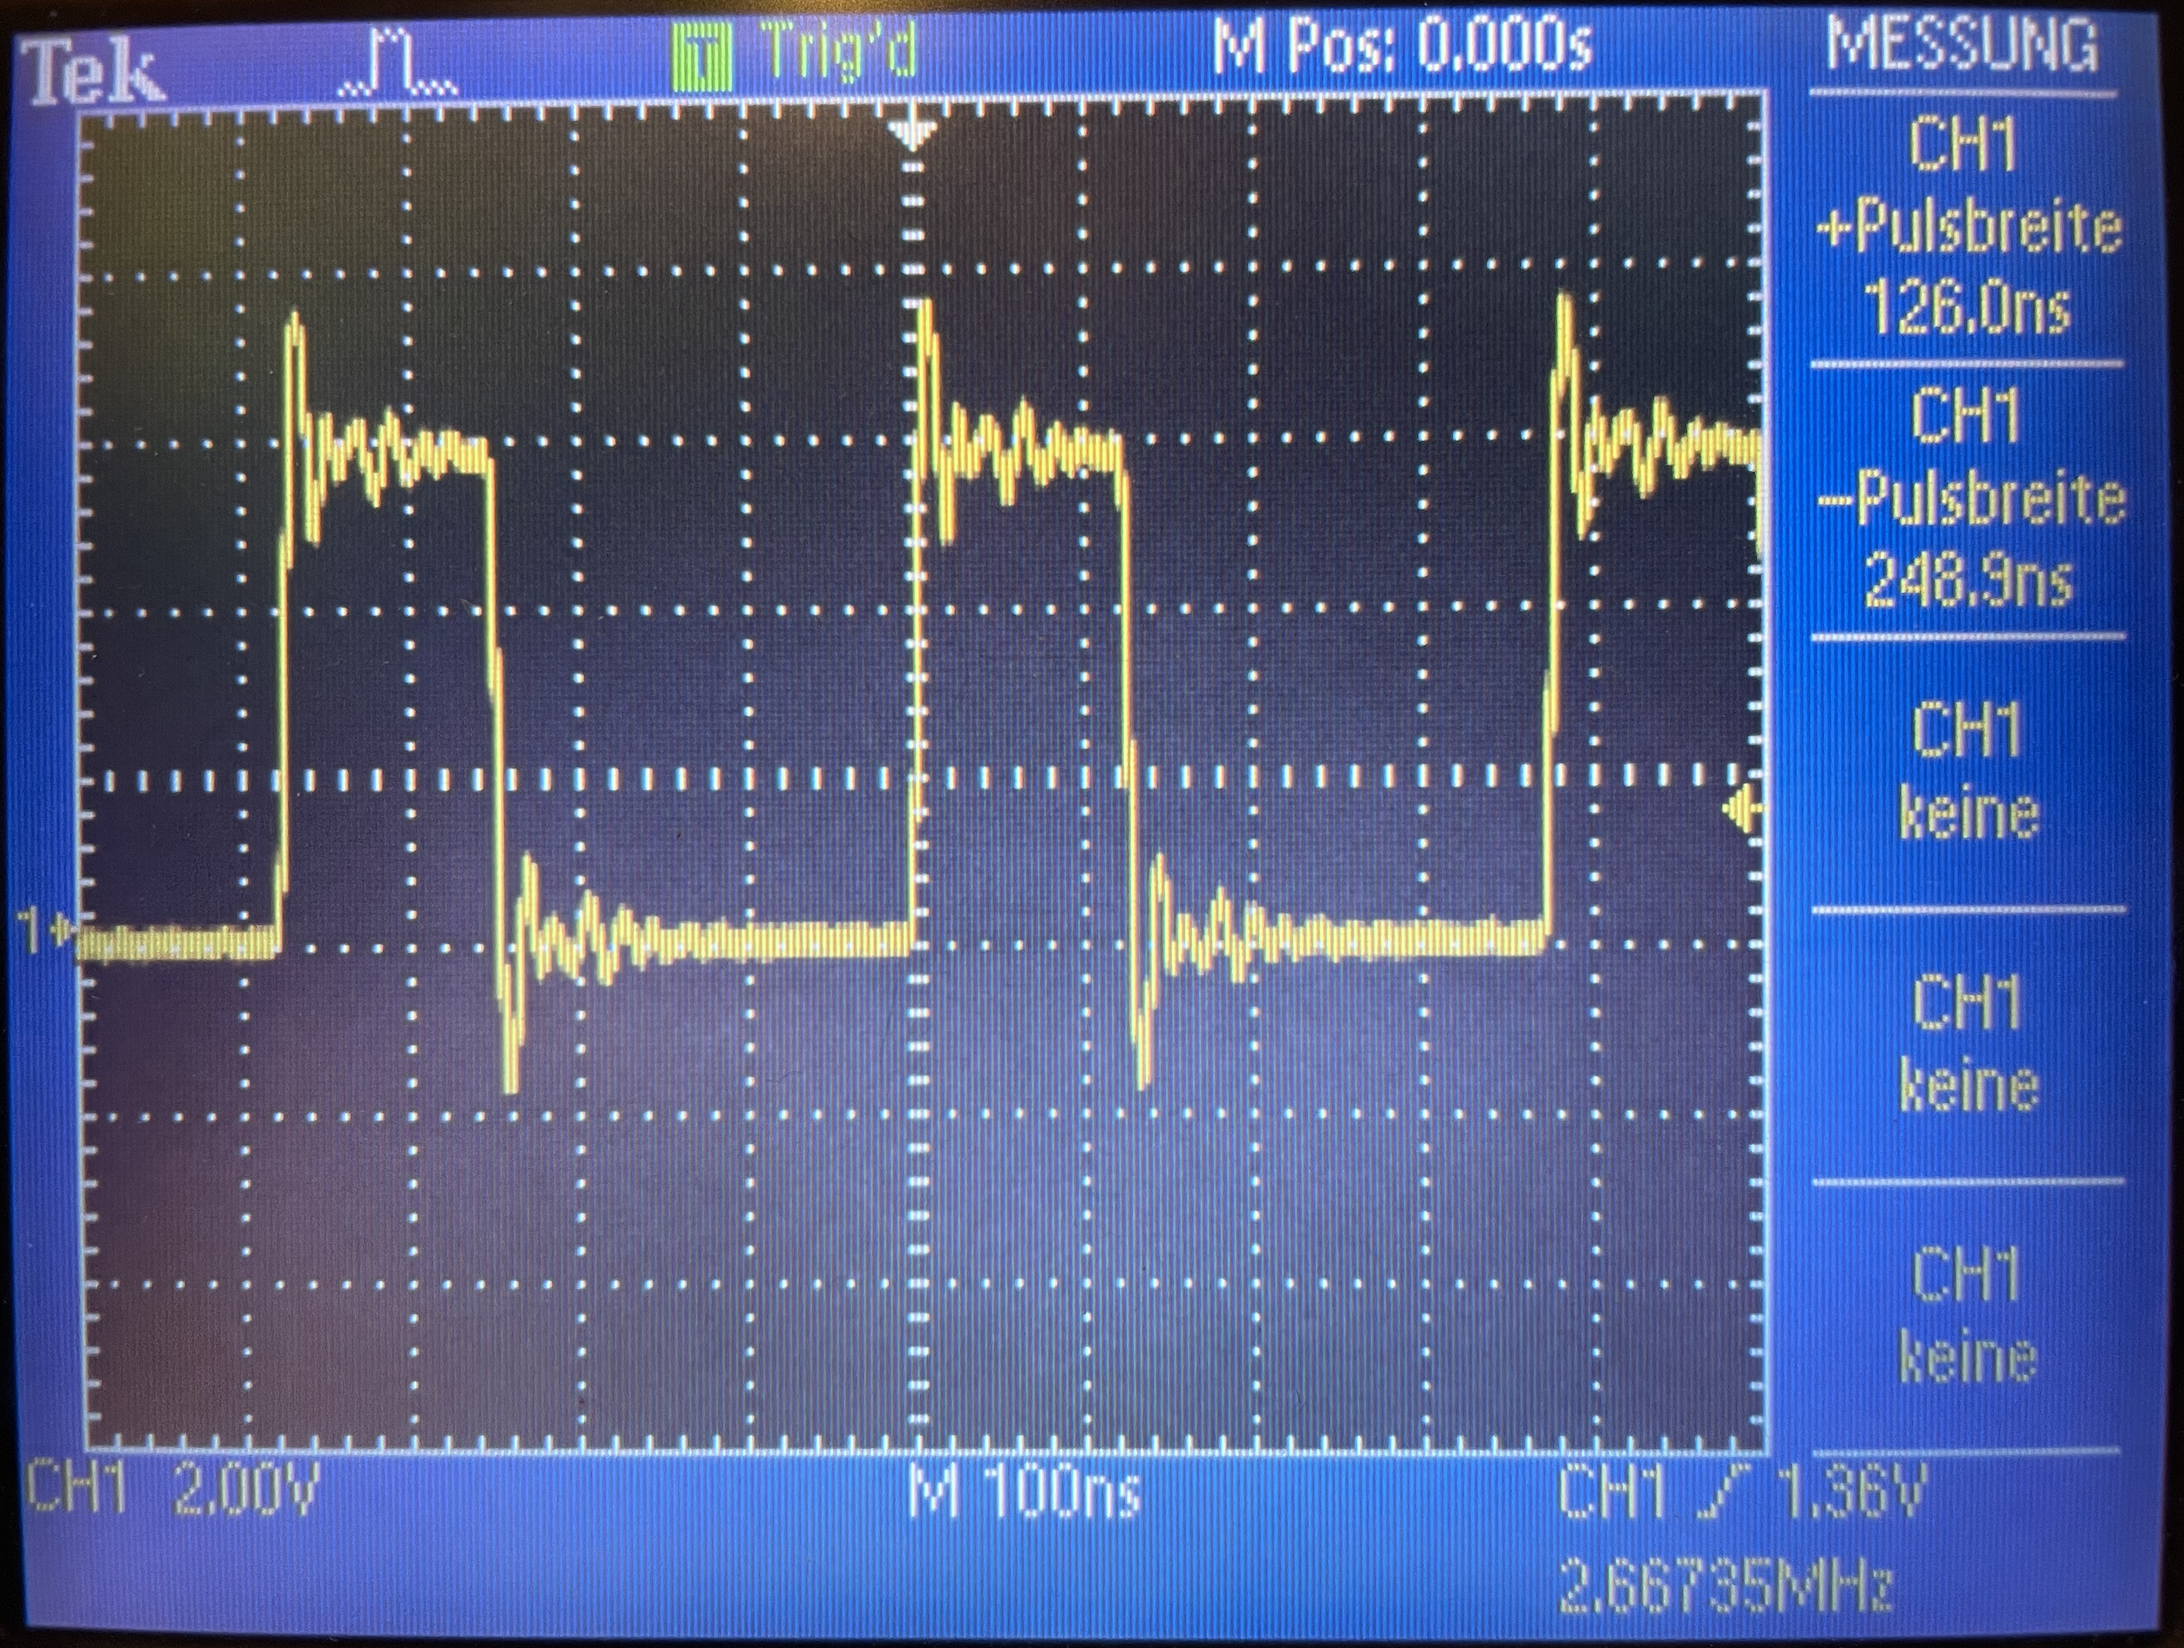
\includegraphics[width=0.8\textwidth]{led-oszi1.png}
    \caption{
	Oszilloskop-Messung an Pin 2 während der Ausführung von
	\texttt{led.hex}.  Die HIGH-Phase dauert etwa 125 ns, die LOW-Phase
	etwa 250 ns – das Signal ist somit nicht symmetrisch.
    }
    \label{fig:led-oszi1}
\end{figure}

\noindent
Zunächst die gute Nachricht: Unser Programm funktioniert wie erwartet – der Pin
wird abwechselnd auf \texttt{HIGH} und \texttt{LOW} gesetzt.

Allerdings zeigt die Messung auch: Das Signal ist nicht symmetrisch. Die
HIGH-Phase dauert nur etwa 125 ns, während die LOW-Phase etwa doppelt so lang
ist. 

Warum das so ist, analysieren wir im nächsten Abschnitt – anhand der internen
Taktzyklen, die jede Instruktion benötigt.

\newpage
\section{Analyse des Programmlaufs}

Der im Labor eingesetzte Mikrocontroller (ATmega328P) arbeitet mit einer
Taktfrequenz von 16 MHz. Damit dauert ein einzelner CPU-Takt:
\[
    \frac{1}{16\,\text{MHz}} = \frac{1}{16 \cdot 10^6}\,\text{s}
    = \frac{1000}{16} \cdot 10^{-9}\,\text{s} = 62.5\,\text{ns}.
\]
Im Datenblatt des ATmega328P kann man nachlesen, wie viele Taktzyklen einzelne
Maschinenbefehle benötigen. Für unser Beispiel ergibt sich eine erfreuliche
Regelmäßigkeit: Jeder der verwendeten Befehle benötigt genau zwei Takte zur
Ausführung – einschließlich des Sprungbefehls.
Wir ergänzen daher unser Ablaufdiagramm um die jeweilige Taktanzahl:

\begin{center}
\begin{tikzpicture}[
	scale=0.8,
	every node/.style={transform shape},
	node distance=0.7cm and 0.8cm
]

\node (step1) [box]
    {Hex: \texttt{52 9a}\\\small Pin 2 als Ausgang benutzen \\\small 2 Takte};
\node (step2) [box, below=of step1]
    {Hex: \texttt{5a 9a}\\\small Pin 2 auf \texttt{HIGH} setzen  \\\small 2 Takte};
\node (step3) [box, below=of step2]
    {Hex: \texttt{5a 98}\\\small Pin 2 auf \texttt{LOW} setzen  \\\small 2 Takte};
\node (step4) [jump, below=of step3]
    {Hex: \texttt{fd cf}\\\small 2 Befehle zurück  \\\small 2 Takte};

\draw [arrow] (step1) -- (step2);
\draw [arrow] (step2) -- (step3);
\draw [arrow] (step3) -- (step4);

% Rücksprungpfeil
\draw [arrow] (step4.east) -- ++(1.5,0) node[right] {} 
              |- (step2.east);

\end{tikzpicture}
\end{center}

\noindent
\hyperref[fig:pin2-takte]{Abbildung~\ref{fig:pin2-takte}} zeigt, wie sich der
Zustand von Pin 2 im Verlauf der Programmausführung verändert.  Beachtet man,
dass zwei CPU-Takte 125 ns und vier Takte 250 ns entsprechen,
erklärt sich damit nicht nur die in
\hyperref[fig:led-oszi1]{Abbildung~\ref{fig:led-oszi1}} gemessene Signalform.
Es zeigt sich auch, dass man durch genaue Kenntnis der Taktanzahl pro Befehl
sehr präzise vorhersagen kann, wie sich das Signal verhalten wird – ganz ohne
zu messen.


\begin{figure}[ht]
\centering
\begin{tikzpicture}[x=0.8cm, y=1cm]

% Achsen
\draw[->] (0,0) -- (14.5,0) node[right] {\footnotesize Takte};
    \draw[->] (0,-0.1) -- (0,1.5) node[above] {\footnotesize Pin 2};

% y-Achse Beschriftung
\draw (0,0) node[left]{LOW};
\draw (0,1) node[left]{HIGH};

% horizontale Hilfslinien
\draw[dashed, gray!40] (0,1) -- (14,1);
\draw[dashed, gray!20] (0,0) -- (14,0);

% Pin-Status
\draw[very thick, myblue]
    (0,0) -- (3.9,0)  % bis inkl. "Pin HIGH"-Befehl = LOW
    -- (4.1,1) -- (5.9,1)  % nach Befehl auf HIGH
    -- (6.1,0) -- (9.9,0) % nach LOW-Befehl wieder LOW
    -- (10.1,1) -- (11.9,1) % HIGH
    -- (12.1,0) -- (14.1,0); % LOW

% vertikale Striche bei jedem Takt
\foreach \x in {0,...,14} {
    \draw[gray!50] (\x, -0.1) -- (\x, 0.1);
    \node[below] at (\x, -0.1) {\tiny \x};
}

% Befehlstexte unter der x-Achse
\newcommand{\annot}[3]{
    \node[font=\footnotesize, align=center, anchor=north] at ({(#1+#2)/2}, -0.5) {#3};
    \draw[gray!50] (#2, -0.55) -- (#2, -1.8);
}

\annot{0}{2}{\texttt{52 9a}\\\tiny Pin 2\\\tiny als Ausgang};
\annot{2}{4}{\texttt{5a 9a}\\\tiny Pin 2\\\tiny HIGH};
\annot{4}{6}{\texttt{5a 98}\\\tiny Pin 2\\\tiny LOW};
\annot{6}{8}{\texttt{fd cf}\\\tiny Sprung};
\annot{8}{10}{\texttt{5a 9a}\\\tiny Pin 2\\\tiny HIGH};
\annot{10}{12}{\texttt{5a 98}\\\tiny Pin 2\\\tiny LOW};
\annot{12}{14}{\texttt{5a 9a}\\\tiny Sprung};

\end{tikzpicture}
\caption{
    Signalverlauf an Pin 2 in Abhängigkeit der CPU-Takte. Die HIGH- und
    LOW-Zustände folgen aus den verwendeten Maschinenbefehlen, die jeweils zwei
    Takte benötigen.
}
\label{fig:pin2-takte}
\end{figure}

\noindent
Im nächsten Abschnitt werden wir das Programm so modifizieren, dass ein
symmetrisches Signal entsteht.


\newpage

\section{Programmanpassung für ein symmetrisches Signal}
\label{sec:Programmanpassung}

Um ein symmetrisches Signal zu erzeugen, müssen wir lediglich dafür sorgen,
dass Pin 2 für zwei zusätzliche Takte auf \texttt{HIGH} bleibt.
Glücklicherweise stellt der ATmega328P – wie nahezu jeder Prozessor – einen
sogenannten \texttt{NOP}-Befehl bereit („No Operation“), der genau das tut:
nichts. Laut Datenblatt benötigt dieser Befehl genau einen CPU-Takt.

Wir können unser bestehendes Programm daher leicht anpassen, indem wir zwei
\texttt{NOP}-Befehle direkt nach dem Setzen von Pin 2 auf \texttt{HIGH}
einfügen. Dadurch bleibt der Pin für insgesamt vier Takte (statt bisher zwei)
auf \texttt{HIGH} und wir erhalten ein symmetrisches Signal mit gleicher Dauer
der \texttt{HIGH}- und \texttt{LOW}-Phasen.
Das neue Ablaufdiagramm sieht wie folgt aus:

\begin{center}
\scalebox{0.7}{%
\begin{tikzpicture}[
	scale=0.8,
	every node/.style={transform shape},
	node distance=0.7cm and 0.8cm
]

\node (step1) [box]
    {Hex: \texttt{52 9a}\\\small Pin 2 als Ausgang benutzen \\\small 2 Takte};
\node (step2) [box, below=of step1]
    {Hex: \texttt{5a 9a}\\\small Pin 2 auf \texttt{HIGH} setzen  \\\small 2 Takte};
\node (step3) [box, below=of step2]
    {Hex: \texttt{00 00}\\\small mache nichts\\\small 1 Takt};
\node (step4) [box, below=of step3]
    {Hex: \texttt{00 00}\\\small mache nichts\\\small 1 Takt};
\node (step5) [box, below=of step4]
    {Hex: \texttt{5a 98}\\\small Pin 2 auf \texttt{LOW} setzen  \\\small 2 Takte};
\node (step6) [jump, below=of step5]
    {Hex: \texttt{fb cf}\\\small 4 Befehle zurück  \\\small 2 Takte};

\draw [arrow] (step1) -- (step2);
\draw [arrow] (step2) -- (step3);
\draw [arrow] (step3) -- (step4);
\draw [arrow] (step4) -- (step5);
\draw [arrow] (step5) -- (step6);

% Rücksprungpfeil
\draw [arrow] (step6.east) -- ++(1.5,0) node[right] {} 
              |- (step2.east);

\end{tikzpicture}
}
\end{center}

\noindent
Schreibt man die Hexadezimalwerte der Befehle nacheinander auf, lautet das
modifizierte Programm:
\begin{center}
    \texttt{52 9a 5a 9a 00 00 00 00 5a 98 fb cf}
\end{center}

\noindent
Zum Abschluss stellt sich nun die Frage, wie das modifizierte Programm in das
Intel-Hex-Format überführt werden kann. Die Herausforderung besteht darin, die
neuen Befehle korrekt in einer Hex-Datei darzustellen, sodass sie von
\texttt{avrdude} fehlerfrei in den Flash-Speicher geschrieben werden können.

\vspace{1em}
\begin{tcolorbox}[colback=myblue!5!white, colframe=myblue, title=Übung]
    Erstelle für das modifizierte Programm eine gültige Intel-Hex-Datei. Achte
    dabei auf die korrekte Adressierung und die richtige Berechnung der
    Prüfsumme. Anschließend kannst du das neue Programm mit \texttt{avrdude}
    auf den Mikrocontroller übertragen und mit dem Oszilloskop überprüfen, ob
    nun ein symmetrisches Signal erzeugt wird.
\end{tcolorbox}

\medskip

\noindent
Wie ihr in diesem Fall die Prüfsumme im Labor unter Gefechtsbedingungen schnell
berechnen könnt, erfahrt ihr auf Laborblatt 1.

%  \begin{center}
%  \ttfamily
%  \colorbox{gray!20}{\strut\textcolor{black}{:}}%
%  \colorbox{myblue!20}{\strut0C}%
%  \colorbox{cyan!20}{\strut0000}%
%  \colorbox{violet!20}{\strut00}%
%  \colorbox{green!10}{\strut529A5A9A000000005A98FBCF}%
%  \colorbox{red!20}{\strut??}
%  \\[0.1cm]
%  \scalebox{0.9}{%
%      \footnotesize
%      \textcolor{myblue}{\textbf{08}} = Länge der Datenbytes,\quad
%      \textcolor{cyan}{\textbf{0000}} = Startadresse,\quad
%      \textcolor{violet}{\textbf{00}} = Record-Typ (Daten),\quad
%      \textcolor{red}{\textbf{5A}} = Prüfsumme
%  }
%  \end{center}

\section{Assembler statt Maschinencode}
\label{sec:led_pin2}

Das bisherige Programm zur Ansteuerung der LED haben wir direkt im
Maschinencode geschrieben – also Byte für Byte festgelegt, welche Instruktionen
ausgeführt werden sollen. Das war eine lehrreiche Erfahrung, aber auch mühsam.
Zum Glück gibt es Werkzeuge, die uns diese Arbeit abnehmen. Ein sogenannter
\emph{Assembler} übersetzt Programme, die in einer menschenlesbaren
Symbolsprache geschrieben sind (sogenannter \emph{Assemblercode}), automatisch
in Maschinencode.  Ein Assemblerprogramm, das exakt dasselbe Verhalten wie
unser modifiziertes LED-Programm erzeugt, könnte folgendermaßen aussehen:

\begin{lstlisting}[
    frame=topbottom,
    caption={Datei \texttt{led\_pin2.s}},
    captionpos=b
]
        sbi     0x0a, 2     ; Pin 2 als Ausgang konfigurieren

loop:   sbi     0x0b, 2     ; Pin 2 auf HIGH setzen
        nop		    ; Nichts machen
        nop		    ; Nichts machen
        cbi     0x0b, 2     ; Pin 2 auf LOW setzen
	rjmp    loop        ; Zurück zur Marke 'loop (d.h. 4 Befehele zurück)
\end{lstlisting}

\noindent
Dabei gilt:
\begin{itemize}
    \item
	\texttt{sbi} steht für „Set Bit“ – ein bestimmtes Bit in einem
	I/O-Register wird auf \texttt{1} gesetzt.
    \item
	\texttt{cbi} steht für „Clear Bit“ – ein bestimmtes Bit wird auf
	\texttt{0} gesetzt.
    \item
	\texttt{nop} ist eine sogenannte No-Operation – der Befehl macht
	nichts, belegt aber einen CPU-Takt.
    \item
	\texttt{rjmp} ist ein relativer Sprungbefehl – er springt um eine
	bestimmte Anzahl an Befehlen zurück (hier: zur Marke \texttt{loop}).
\end{itemize}

\noindent
Der Vorteil: Der Code ist deutlich lesbarer als eine Folge von Bytes wie
\texttt{52 9a ...}. Man erkennt sofort, was gemeint ist – und das Risiko von
Fehlern ist deutlich geringer.

\subsection{Vom Assemblercode zur Intel-Hex-Datei}

Ein Assemblerprogramm wie das oben gezeigte kann mit dem Tool \texttt{avr-as}
in Maschinencode übersetzt werden.  In den guten alten Tagen war das oft schon
alles: Der erzeugte Maschinencode konnte direkt ausgeführt oder als
Intel-Hex-Datei gespeichert werden – fertig.  Die Welt war einfach gestrickt,
und die Werkzeuge ebenso.

Heute sind die Systeme komplexer – und entsprechend auch die Toolchains. Um mit
dieser Komplexität umzugehen, werden die Aufgaben in kleinere Schritte
unterteilt:

\begin{itemize}
    \item
	\texttt{avr-as} erzeugt zunächst eine sogenannte \emph{Objektdatei}
	(\texttt{.o}) mit Maschinencode, aber noch ohne vollständige
	Adressinformationen.
    
    \item
	Diese Datei wird vom \emph{Linker} \texttt{avr-ld} weiterverarbeitet.
        Der Linker ersetzt symbolische Sprungziele – wie zum Beispiel die Marke
        \texttt{loop} in unserem Assemblerprogramm – durch konkrete Adressen.
        Dadurch entsteht eine ausführbare Datei im sogenannten
        \emph{ELF-Format} (Executable and Linkable Format), einem modernen
        Standard unter Linux.

    \item
	Da der ATmega328P das ELF-Format natürlich nicht versteht (er stammt ja
	schließlich aus den guten alten Tagen und er erwartet rohen
	Maschinencode, wie es sich gehört), muss der Maschinencode mit
	\texttt{avr-objcopy} aus der ELF-Datei extrahiert und in das
	\emph{Intel-Hex-Format} überführt werden – ein Format, das sich zum
	Flashen des Mikrocontrollers eignet.

\end{itemize}

\noindent Die komplette Toolchain sieht also so aus:

\begin{lstlisting}
avr-as -o led_pin2.o led_pin2.s
avr-ld -mavr5 -o led_pin2.elf led_pin2.o
avr-objcopy -O ihex -R .eeprom led_pin2.elf led_pin2.hex
\end{lstlisting}

\noindent
\noindent
Bevor man den Mikrocontroller flasht, kann man sich den Inhalt der Datei
\texttt{led\_pin2.hex} ansehen – er sollte exakt mit dem von Hand erzeugten
Intel-Hex-File aus \autoref{sec:Programmanpassung} übereinstimmen. Anschließend
kann der Mikrocontroller – wie bereits in \autoref{sec:avrdude} gezeigt – mit
\texttt{avrdude} geflasht werden.

\subsection{Ein Makefile für Linux und macOS}


\begin{listing}[htbp]
\centering
\caption{
    Datei \texttt{Makefile} zur Übersetzung von Assemblerprogrammen unter Linux
    und macOS. Diese Version verarbeitet ausschließlich \texttt{.s}-Dateien.
}
\label{lst:Makefile_asm}
\vspace{1em}
\begin{minipage}{0.95\textwidth}
\begin{lstlisting}[
    language=make,
    numbers=left,
    numberstyle=\scriptsize,
    stepnumber=1,
    numbersep=4pt,
    basicstyle=\ttfamily\small
]
# Diese Version verarbeitet nur Assemblerprogramme (*.s)
# Später wird ein erweitertes Makefile auch C unterstützen.

SOURCES := $(wildcard *.s)
OBJECTS := $(SOURCES:.s=.o)
ELFS    := $(SOURCES:.s=.elf)
HEXS    := $(SOURCES:.s=.hex)

all: $(HEXS)

%.o: %.s
        avr-as -o $@ $<

%.elf: %.o
        avr-ld -mavr5 -o $@ $<

%.hex: %.elf
        avr-objcopy -O ihex -R .eeprom $< $@

clean:
        $(RM) $(OBJECTS) $(ELFS) $(HEXS)

ifeq ($(MAKECMDGOALS),upload)
ifeq ($(shell uname), Linux)
PORT := $(shell ls /dev/ttyUSB* 2>/dev/null | head -n 1)
else
PORT := $(shell ls /dev/cu.usb* 2>/dev/null | head -n 1)
endif # uname
endif # MAKECMDGOALS == upload

upload: $(HEX)
        @if [ -z "$(HEX)" ]; then \
            echo "Usage: make upload HEX=<filename.hex>"; \
            false; \
        fi
        @if [ -z "$(PORT)" ]; then \
            echo "no USB device found"; \
            false; \
        fi
        avrdude -c arduino -P $(PORT) -p atmega328p -U flash:w:$(HEX):i
\end{lstlisting}
\end{minipage}
\end{listing}

\noindent
Um die Arbeit mit mehreren Assemblerdateien zu erleichtern, verwenden wir das
in \autoref{lst:Makefile_asm} gezeigte \texttt{Makefile}. Dieses sorgt dafür,
dass zu jeder \texttt{.s}-Datei automatisch eine passende Intel-Hex-Datei
erzeugt wird. Das Makefile sollte sich dafür im gleichen Verzeichnis wie die
Assemblerdateien befinden.  Zum Übersetzen genügt der Aufruf:

\begin{lstlisting}
make
\end{lstlisting}
Zusätzlich kann man mit
\begin{lstlisting}
make upload HEX=led_pin2.hex
\end{lstlisting}
gezielt eine Hex-Datei – wie hier \texttt{led\_pin2.hex} – auf den
Mikrocontroller übertragen. Im Prinzip verbirgt sich hinter dem „Verify“-Knopf
in der Arduino-IDE ein Aufruf von \texttt{make}, und hinter dem „Upload“-Knopf
ein Aufruf von \texttt{make upload HEX=\dots}.

\medskip
Für die Übersetzung kommt die zuvor beschriebene Toolchain aus \texttt{avr-as},
\texttt{avr-ld}, \texttt{avr-objcopy} und \texttt{avrdude} zum Einsatz – jedoch
in sinnvoller Kombination. Genauer gesagt:

\begin{itemize}
\item
    Mit \texttt{avr-as} wird \texttt{led\_pin2.o} nur dann erzeugt, wenn sich
    \texttt{led\_pin2.s} verändert hat – also wenn die Quelldatei neuer ist
    als das Objektfile oder letzteres noch fehlt.
\item
    Mit \texttt{avr-ld} wird ein neues \texttt{led\_pin2.elf} nur erzeugt, wenn
    sich \texttt{led\_pin2.o} verändert hat.
\item
    Mit \texttt{avr-objcopy} wird ein neues \texttt{led\_pin2.hex} nur dann
    erzeugt, wenn sich \texttt{led\_pin2.elf} verändert hat.
\end{itemize}

\noindent
Das spart unnötige Arbeit – und genau darin liegt die Stärke von \texttt{make}.
\medskip  
Wird hingegen direkt mit  
\begin{lstlisting}
make upload HEX=led_pin2.hex
\end{lstlisting}  
eine Datei hochgeladen, dann prüft \texttt{make} automatisch, ob die angegebene
Datei aktuell ist – also ob eventuell zuvor noch
Schritte wie die Übersetzung aus \texttt{.s} nach \texttt{.o}, das Linken zur
\texttt{.elf}-Datei oder das Erzeugen der \texttt{.hex}-Datei erforderlich
sind. Auch diese Abhängigkeiten werden zuverlässig erkannt und in der richtigen
Reihenfolge ausgeführt – ganz ohne weiteres Zutun.

Auch wenn man es auf den ersten Blick nicht vermutet:  Was man im
\texttt{Makefile} sieht, ist tatsächlich eine Programmiersprache.  Über deren
Syntax und Benutzerfreundlichkeit lässt sich sicher streiten – aber funktional
ist sie allemal:  Sie erkennt automatisch Abhängigkeiten zwischen Dateien,
entscheidet, welche Zwischenschritte notwendig sind,  und führt sie in der
richtigen Reihenfolge aus.

Allerdings: Manche Dinge tun beim Hinschauen weh – etwa der Block in
Zeile~23--29.  Dass dort die \texttt{ifeq}-Konstrukte nicht eingerückt sind,
ist kein Versehen, sondern leider notwendiger Gehorsam:  \texttt{make}
akzeptiert Direktiven wie \texttt{ifeq}, \texttt{endif}, \texttt{define} usw.\
nur am Zeilenanfang –  genau wie auch einfache Zuweisungen wie
\texttt{PORT~:=~...}.  Eine visuelle Einrückung zur besseren Lesbarkeit ist
schlicht nicht erlaubt.  Gerade wenn man – wie der Autor – allergisch auf
uneinheitliches Einrücken in~C ist  und es für einen Segen hält, dass Python
Einrückung erzwingt,  wirkt die Syntax von \texttt{make} mitunter wie eine
kleine Zeitreise in die 1980er.


Das Makefile in \autoref{lst:Makefile_asm} wird euch im Labor zur Verfügung
gestellt.  Wie man es erweitert, sodass auch C-Programme verarbeitet werden
können, ist später Teil einer Laboraufgabe.
Dazu ist es nicht notwendig, jedes Detail über Makefiles zu kennen.  Es reicht,
wenn ihr zunächst nachvollzieht, wie die oben beschriebenen Abhängigkeiten im
Makefile umgesetzt sind.

In Zeile~11 steht zum Beispiel die Regel, wie man aus einer \texttt{.s}-Datei
eine \texttt{.o}-Datei erzeugt –  sofern eine Aktualisierung notwendig ist
(d.\,h. die \texttt{.o}-Datei fehlt oder älter ist als die zugehörige
\texttt{.s}-Datei).  
In Zeile~12 findet sich mit
\texttt{avr-as -o \$@ \$<} 
das dazugehörige Kommando
wobei \texttt{\$@} automatisch durch den Namen der Zieldatei (also der
\texttt{.o}-Datei) ersetzt wird  und \texttt{\$<} durch den Namen der
Quelldatei (also der \texttt{.s}-Datei).


Insgesamt beschreibt das Makefile somit einen gerichteten Graphen von
Abhängigkeiten, wie er in \autoref{fig:makegraph} visualisiert ist: Jeder
Schritt baut auf dem vorhergehenden auf, und \texttt{make} sorgt dafür, dass
alle nötigen Befehle in der richtigen Reihenfolge ausgeführt werden – aber auch
nur dann, wenn sie wirklich erforderlich sind.


\begin{figure}[ht]
\centering
\begin{tikzpicture}[
  node distance=1.4cm and 3.4cm,
  every node/.style={draw, rounded corners, fill=gray!10, font=\ttfamily},
  arrow/.style={->, thick, >=stealth},
  text height=1.7ex,
  text depth=0pt,
  minimum height=1.8ex,
  align=center
]

\node (s)   {.s};
\node (o)   [right=of s] {.o};
\node (elf) [right=of o] {.elf};
\node (hex) [right=of elf] {.hex};
\node (upload) [below=of hex, yshift=-0.5cm] {upload};

\draw[arrow] (s)   -- (o)     node[midway, above=3pt, fill=myblue!20]  {\small avr-as};
\draw[arrow] (o)   -- (elf)   node[midway, above=3pt, fill=myblue!20]  {\small avr-ld};
\draw[arrow] (elf) -- (hex)   node[midway, above=3pt, fill=myblue!20]  {\small avr-objcopy};
\draw[arrow] (hex) -- (upload) node[midway, right=3pt, fill=myblue!20] {\small avrdude};

\end{tikzpicture}
\caption{
    Abhängigkeitsgraph für die Erzeugung einer \texttt{.hex}-Datei und den
    anschließenden Upload. Die Werkzeuge \texttt{avr-as}, \texttt{avr-ld} und
    \texttt{avr-objcopy} erzeugen die \texttt{.hex}-Datei, die schließlich von
    \texttt{avrdude} auf den Mikrocontroller übertragen wird.
}
\label{fig:makegraph}
\end{figure}


\newpage
\subsection{Eleganter blinken mit exklusivem Oder}

Das folgende Programm lässt – wie zuvor – eine LED blinken, und zwar so, dass
sie abwechselnd 250\,ns an und 250\,ns aus ist. Es entsteht also wieder ein
sauberes, symmetrisches Signal.

Der Unterschied liegt im Code: Diesmal kommen Register zum Einsatz – und vor
allem eine neue Instruktion, nämlich ein exklusives Oder. Diese logische
Operation wird häufig mit \textbf{XOR} abgekürzt (für \emph{exclusive OR}).
Beim ATmega328P heißt die entsprechende Maschineninstruktion jedoch
\textbf{EOR} – wie in Zeile~5 des folgenden Programms.

Werfen wir zuerst einen Blick auf den Code, bevor wir im Detail nachvollziehen,
wie er funktioniert und welche Rolle Register und andere Besonderheiten dabei
spielen:

\begin{lstlisting}[
    frame=topbottom,
    numbers=left,
    numberstyle=\scriptsize,
    caption={Datei \texttt{led\_pin2\_xor.s}},
    captionpos=b,
    label={lst:led_pin2_xor}
]
	ldi	r19,	4	    ; r19 = Maske für Pin 2 (Bem.: 4 = 2^2)
	out	0x0a,	r19	    ; Pin 2 als Ausgang
	ldi	r18,	0	    ; r18 = 0
loop:
	eor	r18,	r19	    ; r18 = r18 XOR r19 ("toggle")
	out	0x0b,	r18	    ; Pin 2 auf HIGH oder LOW setzen
	rjmp	loop
\end{lstlisting}


\medskip
\noindent
Bevor wir den neuen Code Schritt für Schritt analysieren, sollen zunächst
einige wichtige Begriffe und Konzepte geklärt werden:

\begin{itemize}
    \item
	Was sind Register – und worin unterscheiden sie sich von normalen
	Speicherzellen?
    \item
	Was genau sind I/O-Register – und wie kann man über sie die Pins des
	Mikrocontrollers ansteuern?
    \item
	Wie lässt sich ein Pin als Ein- oder Ausgang konfigurieren?
    \item
	Und wie kann man ihn gezielt auf \texttt{HIGH} oder \texttt{LOW}
	setzen?
\end{itemize}
\noindent
Die folgenden Abschnitte beantworten all diese Fragen. Sie helfen nicht nur,
den neuen Code besser zu verstehen, sondern erklären rückblickend auch viele
Details unseres allerersten Assemblerprogramms (\autoref{sec:led_pin2}).

Im Labor könnt ihr übrigens gerne zuerst einfach ausprobieren, ob dieses neue
Programm tatsächlich wieder ein 250\,ns–250\,ns–Blinksignal erzeugt – ganz so
wie das vorherige. Wenn das Oszilloskop ein vertrautes Muster zeigt, ist das
schon mal ein gutes Zeichen. Und wie genau dieses Programm funktioniert, sehen
wir uns jetzt im Detail an.

\paragraph{Register: Rechnen nur mit Register}

Register sind spezielle Speicherzellen, die der Prozessor direkt für
Rechenoperationen verwenden kann. Beim ATmega328P gibt es davon 32 Stück –
jeweils 8~Bit groß – mit den Namen \texttt{r0}, \texttt{r1}, \texttt{r2},
\dots, \texttt{r31}.  Technisch gesehen liegen Register beim ATmega328P im
gleichen Datenraum wie der SRAM (\autoref{fig:speicherarten}), der auch für
lokale und globale Variablen verwendet wird – \textit{die genaue Struktur
dieses Speicherbereichs zeigt} \autoref{fig:sram-struktur}.

\begin{figure}[htbp]
\centering
\begin{center}
\scalebox{0.85}{%
\begin{tikzpicture}
\def\cellsizex{1.2cm}
\def\cellsizey{1cm}

% r0
\draw (0, 0) rectangle ++(\cellsizex, \cellsizey);
\node at (0.5*\cellsizex, 0.5*\cellsizey) {\ttfamily\small r0};
\draw[thick] (0, \cellsizey) -- ++(0, 0.2);
\node[anchor=south] at (0, \cellsizey + 2.5) {\scriptsize 0x00};

% r1
\draw (1*\cellsizex, 0) rectangle ++(\cellsizex, \cellsizey);
\node at (1.5*\cellsizex, 0.5*\cellsizey) {\ttfamily\small r1};
\draw[thick] (1*\cellsizex, \cellsizey) -- ++(0, 0.2);
\node[anchor=south] at (1*\cellsizex, \cellsizey + 2.5) {\scriptsize 0x01};

% Zacken links
\draw[thick]
    (2*\cellsizex, \cellsizey) -- ++(0.125, -0.125)
    -- ++(-0.125, -0.125)
    -- ++(0.125, -0.125)
    -- ++(-0.125, -0.125)
    -- ++(0.125, -0.125)
    -- ++(-0.125, -0.125)
    -- ++(0.125, -0.125)
    -- ++(-0.125, -0.125)
    ;

\node at (2.5*\cellsizex, 0.5*\cellsizey) {\Large\textellipsis};

% Zacken rechts (links von r30)
\draw[thick]
    (3*\cellsizex, \cellsizey) -- ++(-0.125, -0.125)
    -- ++(0.125, -0.125)
    -- ++(-0.125, -0.125)
    -- ++(0.125, -0.125)
    -- ++(-0.125, -0.125)
    -- ++(0.125, -0.125)
    -- ++(-0.125, -0.125)
    -- ++(0.125, -0.125)
    ;

% r30
\draw (3*\cellsizex, 0) rectangle ++(\cellsizex, \cellsizey);
\node at (3.5*\cellsizex, 0.5*\cellsizey) {\ttfamily\small r30};
\draw[thick] (3*\cellsizex, \cellsizey) -- ++(0, 0.2);
\node[anchor=south] at (3*\cellsizex, \cellsizey + 2.5) {\scriptsize 0x1E};

% r31
\draw (4*\cellsizex, 0) rectangle ++(\cellsizex, \cellsizey);
\node at (4.5*\cellsizex, 0.5*\cellsizey) {\ttfamily\small r31};
\draw[thick] (4*\cellsizex, \cellsizey) -- ++(0, 0.2);
\node[anchor=south] at (4*\cellsizex, \cellsizey + 2.5) {\scriptsize 0x1F};


% Klammer mit Beschriftung
\draw [decorate, decoration={brace, mirror, amplitude=6pt}]
      (0*\cellsizex, -0.2) -- (5*\cellsizex, -0.2)
      node[midway, below=6pt, align=center] {\small\textbf{Register}\\\small(0x00 bis 0x1F)};

\draw (5*\cellsizex, 0) rectangle ++(\cellsizex, \cellsizey);
\draw[thick] (5*\cellsizex, \cellsizey) -- ++(0, 0.2);
\node[anchor=south] at (5*\cellsizex, \cellsizey + 2.5) {\scriptsize 0x20};

% Zacken links
\draw[thick]
    (6*\cellsizex, \cellsizey) -- ++(0.125, -0.125)
    -- ++(-0.125, -0.125)
    -- ++(0.125, -0.125)
    -- ++(-0.125, -0.125)
    -- ++(0.125, -0.125)
    -- ++(-0.125, -0.125)
    -- ++(0.125, -0.125)
    -- ++(-0.125, -0.125)
    ;

\node at (6.5*\cellsizex, 0.5*\cellsizey) {\Large\textellipsis};

\draw[thick]
    (7*\cellsizex, \cellsizey) -- ++(-0.125, -0.125)
    -- ++(0.125, -0.125)
    -- ++(-0.125, -0.125)
    -- ++(0.125, -0.125)
    -- ++(-0.125, -0.125)
    -- ++(0.125, -0.125)
    -- ++(-0.125, -0.125)
    -- ++(0.125, -0.125)
    ;
\draw (7*\cellsizex, 0) rectangle ++(\cellsizex, \cellsizey);
\draw[thick] (7*\cellsizex, \cellsizey) -- ++(0, 0.2);
\node at (7.5*\cellsizex, 0.5*\cellsizey) {\ttfamily\small DDRD};
\node[anchor=south] at (7*\cellsizex, \cellsizey + 2.5) {\scriptsize 0x2A};

% Zacken links
\draw[thick]
    (8*\cellsizex, \cellsizey) -- ++(0.125, -0.125)
    -- ++(-0.125, -0.125)
    -- ++(0.125, -0.125)
    -- ++(-0.125, -0.125)
    -- ++(0.125, -0.125)
    -- ++(-0.125, -0.125)
    -- ++(0.125, -0.125)
    -- ++(-0.125, -0.125)
    ;

\node at (8.5*\cellsizex, 0.5*\cellsizey) {\Large\textellipsis};

\draw[thick]
    (9*\cellsizex, \cellsizey) -- ++(-0.125, -0.125)
    -- ++(0.125, -0.125)
    -- ++(-0.125, -0.125)
    -- ++(0.125, -0.125)
    -- ++(-0.125, -0.125)
    -- ++(0.125, -0.125)
    -- ++(-0.125, -0.125)
    -- ++(0.125, -0.125)
    ;
\draw (9*\cellsizex, 0) rectangle ++(\cellsizex, \cellsizey);
\draw[thick] (9*\cellsizex, \cellsizey) -- ++(0, 0.2);
\node at (9.5*\cellsizex, 0.5*\cellsizey) {\ttfamily\small PORTD};
\node[anchor=south] at (9*\cellsizex, \cellsizey + 2.5) {\scriptsize 0x2B};
% Zacken links
\draw[thick]
    (10*\cellsizex, \cellsizey) -- ++(0.125, -0.125)
    -- ++(-0.125, -0.125)
    -- ++(0.125, -0.125)
    -- ++(-0.125, -0.125)
    -- ++(0.125, -0.125)
    -- ++(-0.125, -0.125)
    -- ++(0.125, -0.125)
    -- ++(-0.125, -0.125)
    ;

\node at (10.5*\cellsizex, 0.5*\cellsizey) {\Large\textellipsis};

\draw[thick]
    (11*\cellsizex, \cellsizey) -- ++(-0.125, -0.125)
    -- ++(0.125, -0.125)
    -- ++(-0.125, -0.125)
    -- ++(0.125, -0.125)
    -- ++(-0.125, -0.125)
    -- ++(0.125, -0.125)
    -- ++(-0.125, -0.125)
    -- ++(0.125, -0.125)
    ;
\draw (11*\cellsizex, 0) rectangle ++(\cellsizex, \cellsizey);
\draw[thick] (11*\cellsizex, \cellsizey) -- ++(0, 0.2);
\node[anchor=south] at (11*\cellsizex, \cellsizey + 2.5) {\scriptsize 0x5F};
% Klammer mit Beschriftung
\draw [decorate, decoration={brace, mirror, amplitude=6pt}]
      (5*\cellsizex, -0.2) -- (12*\cellsizex, -0.2)
      node[midway, below=6pt, align=center] {\small\textbf{I/O-Register}\\\small(0x20 bis 0x5F)};


\draw (12*\cellsizex, 0) rectangle ++(\cellsizex, \cellsizey);
\draw[thick] (12*\cellsizex, \cellsizey) -- ++(0, 0.2);
\node[anchor=south] at (12*\cellsizex, \cellsizey + 2.5) {\scriptsize 0x60};
% Zacken links
\draw[thick]
    (13*\cellsizex, \cellsizey) -- ++(0.125, -0.125)
    -- ++(-0.125, -0.125)
    -- ++(0.125, -0.125)
    -- ++(-0.125, -0.125)
    -- ++(0.125, -0.125)
    -- ++(-0.125, -0.125)
    -- ++(0.125, -0.125)
    -- ++(-0.125, -0.125)
    ;

\node at (13.5*\cellsizex, 0.5*\cellsizey) {\Large\textellipsis};

% Zacken rechts (links von r30)
\draw[thick]
    (14*\cellsizex, \cellsizey) -- ++(-0.125, -0.125)
    -- ++(0.125, -0.125)
    -- ++(-0.125, -0.125)
    -- ++(0.125, -0.125)
    -- ++(-0.125, -0.125)
    -- ++(0.125, -0.125)
    -- ++(-0.125, -0.125)
    -- ++(0.125, -0.125)
    ;
\draw (14*\cellsizex, 0) rectangle ++(\cellsizex, \cellsizey);
\draw[thick] (14*\cellsizex, \cellsizey) -- ++(0, 0.2);
\node[anchor=south] at (14*\cellsizex, \cellsizey + 2.5) {\scriptsize 0x85F};

% Klammer mit Beschriftung
\draw [decorate, decoration={brace, mirror, amplitude=6pt}]
      (12*\cellsizex, -0.2) -- (15*\cellsizex, -0.2)
      node[midway, below=6pt, align=center] {\small\textbf{Datenspeicher}\\\small(0x60 bis 0x8FF)};


\end{tikzpicture}
} % scalebox
\end{center}
\caption{
    Schematische Darstellung (nicht maßstabsgetreu) des SRAM-Bereichs des
    ATmega328P. Gezeigt sind die Speicherzellen für die Register, sowie die
    Speicheradressen, mit denen sich die Richtung der Pins festlegen lässt
    (z.\,B. DDRD) oder die Ausgänge direkt gesetzt werden (z.\,B. PORTD).
}
\label{fig:sram-struktur}
\end{figure}

Die Besonderheit ist: Rechenoperationen wie Addition, Vergleich oder logische
Verknüpfungen können ausschließlich mit Registern durchgeführt werden.  Wenn
man mit Variablen arbeiten möchte, die im normalen SRAM liegen, muss man sie
zunächst in ein Register laden – und nach der Berechnung ggf. zurückschreiben.

\noindent
Um überhaupt mit Registern rechnen zu können, müssen sie zunächst mit einem Wert
belegt werden. Eine einfache Möglichkeit dafür ist der Befehl \texttt{ldi}, der
für „load immediate“ steht – auf Deutsch etwa: „direkt laden“. Damit kann man
eine Konstante unmittelbar in ein Register schreiben:

\begin{lstlisting}
    ldi     r19, 4     ; r19 erhält den Wert 4
    ldi     r18, 0     ; r18 erhält den Wert 0
\end{lstlisting}

\noindent
In diesem Beispiel wird das Register \texttt{r19} mit dem Wert \texttt{4}
vorbelegt – also mit einer Bitmaske, bei der nur Bit 2 gesetzt ist. Das Register
\texttt{r18} erhält den Wert \texttt{0}.

Nun kommt eine typische Rechenoperation ins Spiel: die sogenannte
\emph{exklusive Oder}-Verknüpfung (XOR), die im Assembler des ATmega328P durch
den Befehl \texttt{eor} realisiert wird. Sie funktioniert bitweise und liefert
nur dann eine \texttt{1}, wenn die beiden Operanden an der jeweiligen Stelle
unterschiedliche Bits besitzen. Der Befehl

\begin{lstlisting}
    eor     r18, r19
\end{lstlisting}

\noindent
führt dazu, dass der Inhalt von \texttt{r18} durch \texttt{r18 XOR r19}
ersetzt wird. Da \texttt{r18} zuvor den Wert \texttt{0} hatte, und \texttt{r19}
den Wert \texttt{4} hat, ergibt sich \texttt{r18 = 0 XOR 4 = 4}.
Führt man anschließend erneut die Instruktion

\begin{lstlisting}
    eor     r18, r19
\end{lstlisting}

\noindent
aus, dann ist \texttt{r18 = 4 XOR 4 = 0}. Der ursprüngliche Wert wurde also
wieder gelöscht. Wiederholte Anwendung dieser Instruktion toggelt den Inhalt von
\texttt{r18} somit zwischen \texttt{0} und \texttt{4} – genau dieses Verhalten
nutzen wir aus, um den Pin-Zustand wechselweise auf \texttt{HIGH} und
\texttt{LOW} zu setzen:

\begin{center}
\begin{minipage}{0.42\textwidth}
\begin{tikzpicture}[font=\ttfamily]
\node[anchor=west]  at (0,0)     {\phantom{XOR }00000100 \ \ \ \ \ \ (r19 = 4)};
\node[anchor=west]  at (0,-0.6)  {XOR 00000000 \ \ \ \ \ \  (r18 = 0)};
\node[anchor=west]  at (0,-1.1)  {\rule{17em}{0.4pt}};
\node[anchor=west]  at (0,-1.7)  {\phantom{XOR }00000100 \ (neu: r19 = 4)};
\end{tikzpicture}
\end{minipage}
\hfill
\begin{minipage}{0.42\textwidth}
\begin{tikzpicture}[font=\ttfamily]
\node[anchor=west]  at (0,0)     {\phantom{XOR }00000100 \ \ \ \ \ \ (r19 = 4)};
\node[anchor=west]  at (0,-0.6)  {XOR 00000100 \ \ \ \ \ \  (r18 = 4)};
\node[anchor=west]  at (0,-1.1)  {\rule{17em}{0.4pt}};
\node[anchor=west]  at (0,-1.7)  {\phantom{XOR }00000000 \ (neu: r19 = 0)};
\end{tikzpicture}
\end{minipage}
\end{center}

\paragraph{I/O-Register: Schnittstelle zu den Pins}

I/O-Register (Input/Output-Register) sind spezielle Speicherzellen im
SRAM-Bereich, über die sich die Pins des Mikrocontrollers steuern lassen. Für
die Pins~0–7 unseres Mikroprozessors sind vor allem die Adressen \texttt{0x2A}
und \texttt{0x2B} relevant:

\begin{itemize}
    \item
	\texttt{0x2A} entspricht dem sogenannten \texttt{DDRD}-Register. Wenn
	dort das Bit mit Index~2 gesetzt wird, wird Pin~2 als Ausgang
	konfiguriert.
    \item
	\texttt{0x2B} entspricht dem \texttt{PORTD}-Register. Wenn dort das Bit
	mit Index~2 gesetzt wird, liegt an Pin~2 ein HIGH-Pegel an –
	andernfalls ist er LOW.
\end{itemize}

\noindent
Interessant ist: In unserem ersten Assemblerprogramm (siehe
\autoref{sec:led_pin2}) haben wir bereits diese Register verwendet – allerdings
mit anderen Adressen. Dort hieß es zum Beispiel:

\begin{lstlisting}
    sbi     0x0a, 2    ; Pin 2 als Ausgang festlegen
    sbi     0x0b, 2    ; Pin 2 auf HIGH setzen
    cbi     0x0b, 2    ; Pin 2 auf LOW setzen
\end{lstlisting}

\noindent
Hier wurde die Adresse \texttt{0x0a} anstelle von \texttt{0x2A} und
\texttt{0x0b} anstelle von \texttt{0x2B} verwendet.

\noindent
Der Grund: Die Instruktionen \texttt{sbi} (set bit) und \texttt{cbi} (clear
bit) sind speziell dafür gedacht, direkt auf I/O-Register zuzugreifen. Sie
operieren nur auf Adressen im Bereich \texttt{0x00} bis \texttt{0x1F}, was den
ersten 32~I/O-Registern entspricht. Intern wird bei der Ausführung dieser
Befehle automatisch ein Offset von \texttt{0x20} hinzugerechnet. So spart man
im Maschinenbefehl wertvolle Bits, da nur ein kleiner Adressbereich codiert
werden muss.



\paragraph{Ein I/O-Register vollständig überschreiben}

Im bisherigen Beispiel wurden einzelne Bits in den I/O-Registern gezielt
gesetzt oder gelöscht – z.\,B.\ mithilfe der Instruktionen \texttt{sbi} (set
bit) oder \texttt{cbi} (clear bit).  Eine alternative Möglichkeit besteht
darin, gleich das gesamte Register auf einmal zu überschreiben. Das ist nicht
nur kompakter und übersichtlicher, sondern auch effizienter: Während
\texttt{sbi} und \texttt{cbi} jeweils zwei CPU-Takte benötigen, lässt sich ein
vollständiger Schreibzugriff mit der Instruktion \texttt{out} in nur einem
einzigen Takt erledigen.

\medskip
\noindent
Zur Erinnerung:
\begin{itemize}
    \item
	Das Register \texttt{DDRD} (Adresse \texttt{0x2A}) legt fest, welche
	Pins als Ausgang verwendet werden. Um nur Pin~2 als Ausgang zu
	aktivieren, schreibt man die Zahl \texttt{4} (= $2^2$) in das
	\texttt{DDRD}-Register – also genau das Bit mit Index~2.
    \item
	Das Register \texttt{PORTD} (Adresse \texttt{0x2B}) bestimmt, ob ein
	Ausgangspin \texttt{HIGH} oder \texttt{LOW} ist. Um Pin~2 auf
	\texttt{HIGH} zu setzen, schreibt man ebenfalls den Wert \texttt{4}
	hinein. Um ihn auf \texttt{LOW} zu setzen, genügt der Wert \texttt{0}.
\end{itemize}

\medskip
\noindent
Dazu verwendet man die Instruktion \texttt{out}, die zwei Angaben verlangt:
\begin{itemize}
    \item
	die Zieladresse – z.\,B.\ \texttt{0x2A} für \texttt{DDRD} oder
	\texttt{0x2B} für \texttt{PORTD}
    \item
	ein Register, das den zu schreibenden Wert enthält
\end{itemize}
Im folgenden Beispiel wird genau das umgesetzt:
\begin{lstlisting}
    ldi     r19, 4        ; Bit 2 setzen
    out     0x0A, r19     ; Pin 2 als Ausgang festlegen (DDRD)
    out     0x0B, r19     ; Pin 2 auf HIGH setzen (PORTD)
\end{lstlisting}


\noindent
Wichtig: Auch bei \texttt{out} wird – wie bei \texttt{sbi} und \texttt{cbi} –
intern ein Offset von \texttt{0x20} zur angegebenen Adresse addiert. In
obigem Beispiel wird also tatsächlich an Adresse \texttt{0x2A} bzw. an Adresse
\texttt{0x2B} geschrieben, was genau der physikalischen Speicheradresse von
\texttt{DDRD} entspricht (siehe \autoref{fig:sram-struktur}).

\medskip
\noindent
Damit haben wir nun jede Instruktion aus \autoref{lst:led_pin2_xor} verstanden.
Wenn wir jetzt noch den Ablauf des Programms analysieren, wird deutlich, warum
das Signal am Pin 2 erneut symmetrisch ist – also wie beim ersten Programm
jeweils 250\,ns \texttt{HIGH} und 250\,ns \texttt{LOW}. Der folgende Ablaufplan
zeigt die Taktanzahl und erklärt, wie sich der Pin-Zustand über die Zeit ändert:


\begin{center}
\scalebox{0.75}{%
\begin{tikzpicture}[
    scale=0.8,
    every node/.style={transform shape},
    node distance=0.7cm and 0.8cm,
    box/.style={
        rectangle, draw,
        rounded corners,
        minimum width=5.8cm,
        minimum height=1.2cm,
        text centered,
        align=center,
        draw=black,
        fill=gray!10
    }
]

\node (step1) [box]
    {\texttt{ldi r19, 4} \\\small r19 = Maske für Pin 2 ($4 = 2^2$) \\\small 1 Takt};
\node (step2) [box, below=of step1]
    {\texttt{out 0x0a, r19} \\\small Pin 2 als Ausgang \\\small 1 Takt};
\node (step3) [box, below=of step2]
    {\texttt{ldi r18, 0} \\\small r18 = 0 \\\small 1 Takt};
\node (step4) [box, below=of step3]
    {\texttt{eor r18, r19} \\\small r18 = r18 XOR r19 \\\small 1 Takt};
\node (step5) [box, below=of step4]
    {\texttt{out 0x0b, r18} \\\small Pin 2 setzen (HIGH/LOW) \\\small 1 Takt};
\node (step6) [jump, below=of step5]
    {\texttt{rjmp loop} \\\small zurück zu \texttt{eor r18, r19} \\\small 2 Takte};

\draw [arrow] (step1) -- (step2);
\draw [arrow] (step2) -- (step3);
\draw [arrow] (step3) -- (step4);
\draw [arrow] (step4) -- (step5);
\draw [arrow] (step5) -- (step6);

% Rücksprung
\draw [arrow] (step6.east) -- ++(1.5,0) node[right] {}
              |- (step4.east);

\end{tikzpicture}
}
\end{center}


\newpage
\section{Einfaches Delay mit einem Register}

Unser nächstes Ziel ist es, dass Pin 2 etwas langsamer zwischen HIGH und LOW
wechselt. Am Ende soll es schließlich möglich sein, dort eine LED
anzuschließen, die dann für das Auge wahrnehmbar mit einer vorgegebenen
Frequenz blinkt. 

Kleiner Spoiler: Mit dem aktuellen Ansatz würde die LED mit etwa 20 000 Hertz
blinken – das wäre für das Auge immer noch nicht wahrnehmbar (selbst wenn es
technisch möglich wäre, eine LED mit so hoher Frequenz ein- und auszuschalten). 

Aber die Idee, die wir hier entwickeln und umsetzen, lässt sich leicht
verbessern, um im nächsten Abschnitt unser Ziel zu erreichen.
Der in \autoref{lst:led_pin2_delay1} gezeigte Code enthält im Vergleich zu
\autoref{lst:led_pin2_xor} drei zusätzliche Instruktionen, die in den Zeilen 7
bis 10 hinzugekommen sind:

\begin{itemize}
    \item
	Die Instruktion in Zeile~7 initialisiert das Register \texttt{r24} mit
	dem Wert~2. Dieses Register dient als Zähler für einen Countdown und
	kann natürlich auch mit anderen Werten belegt werden. Da Register bei
	unserem Mikrocontroller jedoch nur 8~Bit breit sind, sind nur Werte von
	\texttt{0} bis \texttt{255} (bzw.\ in Hexadezimaldarstellung von
	\texttt{0x00} bis \texttt{0xFF}) möglich.
  
    \item
	Die Instruktion in Zeile~9 dekrementiert das Register \texttt{r24}
	um~1. Technisch wird dabei der Wert \texttt{1} von \texttt{r24}
	subtrahiert und das Ergebnis wieder in \texttt{r24} gespeichert.
	Wichtig ist hierbei, dass bei dieser Subtraktion nicht nur das
	Rechenergebnis, sondern auch sogenannte \emph{Statusflags} berechnet
	werden. Eines davon ist das sogenannte \emph{Zero-Flag}, das genau dann
	gesetzt wird, wenn das Ergebnis der Subtraktion gleich~0 ist.
  
    \item
	Die Instruktion in Zeile~10 ist ein bedingter Sprung. \texttt{brne}
	steht für \enquote{Branch if Not Equal} und bedeutet: Der Sprung zur
	Marke \texttt{delay} erfolgt nur, wenn das Zero-Flag \emph{nicht}
	gesetzt ist – also genau dann, wenn \texttt{r24} nach der letzten
	Subtraktion noch nicht~0 ist. Ist das Zero-Flag hingegen gesetzt
	(d.\,h. \texttt{r24} ist jetzt~0), wird mit der nächsten Instruktion in
	Zeile~12 fortgefahren.
\end{itemize}

\noindent
\autoref{fig:delay1} zeigt ein Ablaufdiagramm für das Programm in
\autoref{lst:led_pin2_delay1}. Hier wird deutlich, dass mit den neu eingefügten
Zeilen eine innere Schleife realisiert wird, in der das Register \texttt{r24}
heruntergezählt wird. Diese Schleife ist eingebettet in eine äußere Schleife,
mit der Pin~2 abwechselnd auf \texttt{HIGH} und \texttt{LOW} gesetzt wird.

Je größer der initiale Wert von \texttt{r24} ist, desto mehr Takte werden
benötigt, um die innere Schleife zu durchlaufen, bevor erneut der Zustand von
Pin~2 geändert wird. Die Dauer, die Pin~2 in einem bestimmten Zustand (also
\texttt{HIGH} oder \texttt{LOW}) verweilt, lässt sich somit gezielt
beeinflussen.


\begin{listing}[htbp]
\begin{lstlisting}[
    frame=topbottom,
    numbers=left,
    numberstyle=\scriptsize,
    caption={
	\texttt{led\_pin2\_delay1.s} – Pin 2 wird mit Hilfe einer
	Countdown-Schleife in \texttt{r24} verzögert getoggelt
    },
    captionpos=b,
    label={lst:led_pin2_delay1}
]
        ldi     r19,    4           ; 1 Takt
        out     0x0a,   r19         ; 1 Takt
        ldi     r18,    0           ; 1 takt
loop:
        eor     r18,    r19         ; 1 Takt
        out     0x0b,   r18         ; 1 Takt
	ldi     r24,    0x2         ; 1 Takt (Zähler für Countdown setzen)
delay:
        subi    r24,    1           ; 1 Takt
        brne    delay               ; 2 Takte bei Sprung, 1 Takt sonst

        rjmp    loop                ; 2 Takte
\end{lstlisting}
\end{listing}

\begin{figure}[htbp]
\centering
\begin{center}
\scalebox{0.75}{%
\begin{tikzpicture}[
    scale=0.8,
    every node/.style={transform shape},
    node distance=0.7cm and 0.8cm,
    box/.style={
        rectangle, draw,
        rounded corners,
        minimum width=5.8cm,
        minimum height=1.2cm,
        text centered,
        align=center,
        draw=black,
        fill=gray!10
    }
]
\node (step1) [box]
    {
	\texttt{ldi r19, 4} \\
	\small r19 = Maske für Pin 2 ($4 = 2^2$) \\
	\small 1 Takt
    };
\node (step2) [box, below=of step1]
    {
	\texttt{out 0x0a, r19} \\
	\small Pin 2 als Ausgang \\
	\small 1 Takt
    };
\node (step3) [box, below=of step2]
    {
	\texttt{ldi r18, 0} \\
	\small r18 = 0 \\
	\small 1 Takt
    };
\node (step4) [box, below=of step3]
    {
	\texttt{eor r18, r19} \\
	\small r18 = r18 XOR r19 \\
	\small 1 Takt
    };
\node (step5) [box, below=of step4]
    {
	\texttt{out 0x0b, r18} \\
	\small Pin 2 setzen (HIGH/LOW) \\
	\small 1 Takt
    };
\node (step6) [box, below=of step5]
    {
	\texttt{ldi r24, 0x02} \\
	\small r24 = 0x02 (Zähler, hier $n=2$)\\
	\small 1 Takt
    };
\node (step7) [box, below=of step6]
    {
	\texttt{subi r24, 1} \\
	\small r24 = r24 - 1 \\
	\small 1 Takt
    };
\node (step8) [jump, below=of step7]
    {
	\texttt{brne    delay} \\
	\small Zurück, falls r24 \neq 0 (2 Takte)\\
	\small Sonst weiter (1 Takt)
    };
\node (step9) [jump, below=of step8]
    {
	\texttt{rjmp loop} \\
	\small zurück zu \texttt{eor r18, r19} \\
	\small 2 Takte
    };
\draw [arrow] (step1) -- (step2);
\draw [arrow] (step2) -- (step3);
\draw [arrow] (step3) -- (step4);
\draw [arrow] (step4) -- (step5);
\draw [arrow] (step5) -- (step6);
\draw [arrow] (step6) -- (step7);
\draw [arrow] (step7) -- (step8);
\draw [arrow] (step8) -- (step9) node[midway, right] {\small falls r24 = 0};

% Rücksprung
\draw [arrow] (step8.east) -- ++(2.5,0)
	      |- (step7.east) node[midway, above] {\small falls r24 $\neq$ 0};
\draw [arrow] (step9.east) -- ++(5.5,0) node[right] {}
	      |- (step4.east);

\end{tikzpicture}
}
\end{center}
\caption{
    Ablaufdiagramm für das Programm aus \autoref{lst:led_pin2_delay1} mit
    Verzögerungsschleife über \texttt{r24}. Die äußere Schleife ändert den
    Pin-Zustand, die innere Schleife erzeugt eine variable Pause.
}
\label{fig:delay1}
\end{figure}

\subsection{Taktanzahl pro Schleifendurchlauf}

Wir möchten nun berechnen, wie viele Takte zwischen zwei aufeinanderfolgenden
Ausführungen der \texttt{eor}-Instruktion in Zeile~5 vergehen – also wie lange
es dauert, bis sich der Zustand von Pin~2 wieder ändert.

Entscheidend ist dabei, wie oft die innere Schleife durchlaufen wird. Wenn das
Register \texttt{r24} mit einem Wert \( n \) initialisiert wird, dann wird die
Schleife insgesamt \( n \) Mal durchlaufen. Dabei erfolgt der Rücksprung zur
Marke \texttt{delay} genau \( n-1 \) Mal. Beim \( n \)-ten Mal ist das Ergebnis
der Subtraktion null, das Zero-Flag ist gesetzt, und es erfolgt kein Sprung
mehr.

\noindent
Laut Datenblatt benötigt die \texttt{subi}-Instruktion (Zeile~9) stets 1
Takt.  Die \texttt{brne}-Instruktion (Zeile~10) benötigt:
\begin{itemize}
  \item 2 Takte, wenn der Sprung ausgeführt wird (\( n-1 \) Mal),
  \item 1 Takt, wenn kein Sprung erfolgt (1 Mal).
\end{itemize}
Die innere Schleife (Zeilen~9–10) benötigt damit insgesamt:
\[
(n-1) \cdot (1 + 2) + 1 + 1 = 3(n-1) + 2 \quad \text{Takte}
\]
Zusätzlich werden vor und nach dieser Schleife folgende Instruktionen
ausgeführt:
\begin{itemize}
  \item Zeile~6: \texttt{ldi r24, n} → 1 Takt
  \item Zeile~5: \texttt{out 0x0b, r18} → 1 Takt
  \item Zeile~4: \texttt{eor r18, r19} → 1 Takt
  \item Zeile~11: \texttt{rjmp loop} → 2 Takte
\end{itemize}
Das ergibt insgesamt:
\[
3(n-1) + 2 + 3 + 2 = 3n + 4 \quad \text{Takte pro Schleifendurchlauf.}
\]
Je größer also der Initialwert \( n \), desto länger dauert es, bis sich der
Zustand an Pin~2 wieder ändert.


\subsection{Nachmessen der Verzögerung}

Die folgende Tabelle zeigt, wie viele Takte für einen Durchlauf der äußeren
Schleife benötigt werden, abhängig vom Initialwert \( n \) im Register
\texttt{r24}. Die Anzahl der Takte ergibt sich gemäß der vorherigen Herleitung
zu:
\begin{equation}
    \label{eq:delay1}
    T(n) = 3(n - 1) + 7 = 3n + 4
\end{equation}
Ein Takt dauert bei einem Mikrocontroller mit 16\,MHz genau
\( \SI{62.5}{\nano\second} \). 
\autoref{tab:delaytimes} zeigt für verschiedene Werte von \( n \), wie viele
Takte und wie viel Zeit ein kompletter Durchlauf der äußeren Schleife benötigt.
Natürlich werden wir das im Labor nachmessen. Dabei ist es hilfreich, zunächst
für kleine Werte von \( n \) zu überprüfen, wie lange Pin 2 jeweils auf HIGH
bzw. LOW ist, um so die Formel aus \eqref{eq:delay1} zu validieren.

\begin{table}[H]
\centering
\begin{tabular}{c c c c}
\toprule
Initialwert \( n \) & Taktanzahl & Zeit in \si{\micro\second} & Zeit in \si{\nano\second} \\
\midrule
1   & 7   & 0{,}4375  & 437{,}5 \\
2   & 10  & 0{,}6250  & 625 \\
3   & 13  & 0{,}8125  & 812{,}5 \\
4   & 16  & 1{,}0000  & 1000 \\
255 & 769 & 48{,}0625 & 48062{,}5 \\
\bottomrule
\end{tabular}
\caption{Verzögerung pro Schleifendurchlauf für verschiedene Initialwerte}
\label{tab:delaytimes}
\end{table}


\newpage
\section{Längeres Delay mit vier Registern}

\begin{listing}[htbp]
\begin{lstlisting}[
    frame=topbottom,
    numbers=left,
    numberstyle=\scriptsize,
    caption={
	Programm \texttt{led\_pin2\_delay4.s}: Vier Register
	(\texttt{r24} bis \texttt{r27}) werden als 32-Bit-Zähler verwendet,
	um ein deutlich längeres Delay zu erzeugen. Der Pin 2 wird dabei
	weiterhin mit jeder Iteration der äußeren Schleife getoggelt.
    },
    captionpos=b,
    label={lst:led_pin2_delay4}
]
        ldi     r19,    4           ; für Pin 2 (4 = 2^2)
        out     0x0a,   r19
        ldi     r18,    0
loop:
        eor     r18,    r19         ; 1 Takt
        out     0x0b,   r18         ; 1 Takt

        ldi     r24,    0x54        ; 1 Takt
        ldi     r25,    0x58        ; 1 Takt
        ldi     r26,    0x14        ; 1 Takt
        ldi     r27,    0x00        ; 1 Takt
delay:
        subi    r24,    1           ; 1 Takt
        sbci    r25,    0           ; 1 Takt
        sbci    r26,    0           ; 1 Takt
        sbci    r27,    0           ; 1 Takt
        brne    delay               ; 2 Takte bei Sprung, 1 Takt sonst

        rjmp    loop                ; 2 Takte
\end{lstlisting}
\end{listing}


\noindent
Um ein längeres Delay zu erzielen, benötigen wir mehr als 8 Bit für den
Countdown-Zähler. Das in \autoref{lst:led_pin2_delay4} gezeigte Programm
verwendet daher einen 32-Bit-Zähler, der über die vier Register \texttt{r24}
bis \texttt{r27} realisiert wird. Diese werden als Registerverbund betrachtet
und gemeinsam heruntergezählt, um eine deutlich längere Verzögerung zu
erreichen als mit nur einem einzelnen Register.

Ein \emph{Registerverbund} bezeichnet die Interpretation mehrerer
aufeinanderfolgender 8-Bit-Register als ein gemeinsames größeres Register, in
unserem Fall ein 32-Bit-Zähler. Jedes Register speichert dabei ein Byte des
Gesamtwerts, wobei \texttt{r24} das niederwertigste Byte und \texttt{r27} das
höchstwertige Byte enthält. Zum Beispiel entspricht die folgende Belegung

\begin{center}
    \texttt{r24 = 0x12}, \quad \texttt{r25 = 0x34},
    \quad \texttt{r26 = 0x56}, \quad \texttt{r27 = 0x78}
\end{center}

\noindent
dem zusammengesetzten Wert
\[
    n = \texttt{r27:r26:r25:r24} = \texttt{0x78563412}.
\]
Im Listing \autoref{lst:led_pin2_delay4} wird der Zähler in den Zeilen 8 bis 11
mit vier \texttt{ldi}-Instruktionen initialisiert. Dort ergibt sich
\[
    n = \texttt{r27:r26:r25:r24} = \texttt{0x00000200} = 512,
\]
was bedeutet, dass die Schleife 512-mal durchlaufen wird, bevor der Zustand von
Pin 2 erneut geändert wird.

\noindent
Bei unserem Mikroprozessor gibt es keine Instruktion, um direkt einen
Registerverbund mit vier Registern zu dekrementieren%
\footnote{Für einen Registerverbund aus zwei Registern,
z.\,B.\ \texttt{r25:r24}, gibt es die \texttt{SBIW}-Instruktion
(Subtract Immediate from Word).}. 
Man kann eine solche Operation aber durch eine Kombination von \texttt{subi}
(Subtrahiere Sofortwert) und \texttt{sbci} (Subtrahiere mit Übertrag)
nachbauen. Das geschieht in den Zeilen~13 bis~16
in \autoref{lst:led_pin2_delay4}:

\begin{lstlisting}[language={},numbers=none]
        subi    r24,    1
        sbci    r25,    0
        sbci    r26,    0
        sbci    r27,    0
\end{lstlisting}

\noindent
Vereinfacht gesagt haben diese vier Instruktionen den Effekt, dass der gesamte
32-Bit-Wert im Registerverbund \texttt{r27:r26:r25:r24} um eins dekrementiert
wird. Sobald der Wert den Wert Null erreicht hat (d.\,h.\ alle vier Register
enthalten den Wert \texttt{0x00}), wird das Zero-Flag im Statusregister gesetzt
– andernfalls bleibt es gelöscht.

\vspace{1em}
\noindent
\textbf{Etwas genauer:} Die \texttt{subi}-Instruktion subtrahiert
den Wert~1 von \texttt{r24} und setzt dabei die Flags im Statusregister, unter
anderem das Carry-Flag (C), falls ein Übertrag stattgefunden hat. Zwei typische
Fälle:
\begin{itemize}
    \item
	\textbf{Fall 1:} \texttt{r24 = 0x01} vor der Subtraktion.\\
	Nach \texttt{subi r24, 1} ist \texttt{r24 = 0x00}, und es tritt kein
	Übertrag auf, das Carry-Flag bleibt gelöscht.
    \item
	\textbf{Fall 2:} \texttt{r24 = 0x00} vor der Subtraktion.\\
	Nach \texttt{subi r24, 1} ergibt sich \texttt{r24 = 0xFF}, da die
	Subtraktion unterläuft. In diesem Fall wird das Carry-Flag gesetzt.
\end{itemize}
Allgemein gilt: Das Carry-Flag wird bei \texttt{subi} genau dann gesetzt, wenn
\texttt{r24} vor der Subtraktion den Wert \texttt{0x00} hatte, also ein
Übertrag beim Subtrahieren von 1 auftritt.

Die nachfolgenden \texttt{sbci}-Instruktionen subtrahieren dann jeweils den
Wert~0 \emph{unter Berücksichtigung} des Carry-Flags. Wenn es z.\,B.\ beim
Dekrementieren von \texttt{r24} einen Übertrag gab (weil es vorher 0 war), wird
dieser Übertrag auf \texttt{r25} übertragen, wodurch der Verbund korrekt um 1
dekrementiert wird. Die Verkettung dieser vier Instruktionen bildet damit ein
korrektes 32-Bit-Dekrement nach.
Das Zero-Flag wird nur dann gesetzt, wenn das Ergebnis der gesamten Operation
null ist, d.\,h.\ alle vier Register enthalten \texttt{0x00} und es gab keinen
Übertrag mehr nach der letzten \texttt{sbci}-Instruktion.

\subsection{Taktanzahl pro Schleifendurchlauf}

\autoref{fig:delay4} zeigt ein Ablaufdiagramm für \autoref{lst:led_pin2_delay4}. 
Obwohl wir deutlich mehr Instruktionen haben als beim Delay mit einem Register, 
ist die Struktur sehr ähnlich: Eine innere Schleife für die Verzögerung und 
eine äußere für das Togglen von Pin 2.

Wir können also analog bestimmen, wie viele Takte vergehen, 
bis sich der Zustand von Pin 2 wieder ändert. 
Ist \( n \) der Wert des Register-Verbunds \texttt{r27:r26:r25:r24}, 
dann benötigt die innere Schleife
\[
    (n - 1) \cdot 6 + 5
\]
Takte. Die äußere Schleife enthält weitere Instruktionen, 
die zusammen 8 Takte benötigen. Insgesamt ergibt sich damit:
\[
    T(n) = (n - 1) \cdot 6 + 5 + 8 = 6n + 7
\]
Für einige Beispielwerte lässt sich das überprüfen:
\begin{itemize}
    \item
	\( n = 1 \Rightarrow T(1) = 13 \) Takte
	\( \Rightarrow 13 \cdot 62{,}5\,\text{ns} = 812{,}5\,\text{ns} \)
    \item
	\( n = 2 \Rightarrow T(2) = 19 \) Takte
	\( \Rightarrow 19 \cdot 62{,}5\,\text{ns} = 1187{,}5\,\text{ns} \)
\end{itemize}
Noch interessanter ist die Frage, welchen Wert \( n \) man wählen muss, 
damit Pin 2 mit einer Frequenz von 1 Hz blinkt, also jeweils 500 ms HIGH und
500 ms LOW ist.  Dazu muss gelten:
\[
    (6n + 7) \cdot 62{,}5\,\text{ns}
	= 500\,\text{ms} = 500\,000\,000\,\text{ns}
\]
Löst man diese Gleichung nach \( n \) auf, ergibt sich:
\[
    n = \frac{500\,000\,000 / 62{,}5 - 7}{6}
	= \frac{8\,000\,000 - 7}{6} = 1\,333\,332{,}166\ldots
\]
Da wir nur ganze Werte für \( n \) einsetzen können, wählen wir:
\[
n = 1\,333\,332 = \texttt{0x145854}
\]
Dieser Wert liegt innerhalb unserer Messgenauigkeit und 
sorgt dafür, dass eine angeschlossene LED etwa mit 1 Hz blinkt.


\begin{figure}[htbp]
\centering
\begin{center}
\scalebox{0.75}{%
\begin{tikzpicture}[
    scale=0.8,
    every node/.style={transform shape},
    node distance=0.5cm and 0.7cm,
    box/.style={
        rectangle, draw,
        rounded corners,
        minimum width=5.8cm,
        minimum height=1.2cm,
        text centered,
        align=center,
        draw=black,
        fill=gray!10
    }
]
\node (step1) [box]
    {
	\texttt{ldi r19, 4} \\
	\small r19 = Maske für Pin 2 ($4 = 2^2$) \\
	\small 1 Takt
    };
\node (step2) [box, below=of step1]
    {
	\texttt{out 0x0a, r19} \\
	\small Pin 2 als Ausgang \\
	\small 1 Takt
    };
\node (step3) [box, below=of step2]
    {
	\texttt{ldi r18, 0} \\
	\small r18 = 0 \\
	\small 1 Takt
    };
\node (step4) [box, below=of step3]
    {
	\texttt{eor r18, r19} \\
	\small r18 = r18 XOR r19 \\
	\small 1 Takt
    };
\node (step5) [box, below=of step4]
    {
	\texttt{out 0x0b, r18} \\
	\small Pin 2 setzen (HIGH/LOW) \\
	\small 1 Takt
    };
\node (step6) [box, below=of step5]
    {
	\texttt{ldi r24, 0x00} \\
	\small r24 = 0x00\\
	\small 1 Takt
    };
\node (step7) [box, below=of step6]
    {
	\texttt{ldi r25, 0x02} \\
	\small r25 = 0x02\\
	\small 1 Takt
    };
\node (step8) [box, below=of step7]
    {
	\texttt{ldi r26, 0x00} \\
	\small r26 = 0x02\\
	\small 1 Takt
    };
\node (step9) [box, below=of step8]
    {
	\texttt{ldi r27, 0x00} \\
	\small r27 = 0x02\\
	\small 1 Takt
    };
\node (step10) [box, below=of step9]
    {
	\texttt{subi r24, 1} \\
	\small r24 = r24 - 1 \\
	\small 1 Takt
    };
\node (step11) [box, below=of step10]
    {
	\texttt{sbci r25, 1} \\
	\small r25 = r25 - voriger Überlauf  \\
	\small 1 Takt
    };
\node (step12) [box, below=of step11]
    {
	\texttt{sbci r26, 1} \\
	\small r26 = r26 - voriger Überlauf  \\
	\small 1 Takt
    };
\node (step13) [box, below=of step12]
    {
	\texttt{sbci r27, 1} \\
	\small r27 = r27 - voriger Überlauf  \\
	\small 1 Takt
    };
\node (step14) [jump, below=of step13]
    {
	\texttt{brne    delay} \\
	\small Zurück, falls r27:r26:r25:r24 \neq 0 (2 Takte)\\
	\small Sonst weiter (1 Takt)
    };
\node (step15) [jump, below=of step14]
    {
	\texttt{rjmp loop} \\
	\small zurück zu \texttt{eor r18, r19} \\
	\small 2 Takte
    };
\draw [arrow] (step1) -- (step2);
\draw [arrow] (step2) -- (step3);
\draw [arrow] (step3) -- (step4);
\draw [arrow] (step4) -- (step5);
\draw [arrow] (step5) -- (step6);
\draw [arrow] (step6) -- (step7);
\draw [arrow] (step7) -- (step8);
\draw [arrow] (step8) -- (step9);
\draw [arrow] (step9) -- (step10);
\draw [arrow] (step10) -- (step11);
\draw [arrow] (step11) -- (step12);
\draw [arrow] (step12) -- (step13);
\draw [arrow] (step13) -- (step14);
\draw [arrow] (step14) -- (step15) node[midway, right]
    {\small falls  r27r26r25r24 = 0};

% Rücksprung
\draw [arrow] (step14.east) -- ++(2.5,0)
	      |- (step10.east) node[midway, above]
		{\small falls r27:r26:r25:r24 $\neq$ 0};
\draw [arrow] (step15.east) -- ++(7.5,0) node[right] {}
	      |- (step4.east);

\end{tikzpicture}
}
\end{center}
\caption{
    Ablaufdiagramm zum Programm \texttt{led\_pin2\_delay4.s}. Der Countdown
    erfolgt über einen 32-Bit-Registerverbund (\texttt{r27:r26:r25:r24}). Das
    Diagramm zeigt, wie durch die innere Schleife mi
    t \texttt{subi}/\texttt{sbci}/\texttt{brne} ein längeres Delay erzeugt
    wird, bevor in der äußeren Schleife der Zustand von Pin 2 erneut
    gewechselt wird.
}
\label{fig:delay4}
\end{figure}


\newpage
\section{Bare-Metal-C}

\begin{listing}[htbp]
\begin{lstlisting}[
    frame=topbottom,
    numbers=left,
    numberstyle=\scriptsize,
    caption={
	C-Programm \texttt{led\_pin2\_delay.c}, das nahezu identischen
	Assembler-Code erzeugt wie die handgeschriebene Variante in
	\autoref{lst:led_pin2_delay4}.
	Die LED an Pin 2 wird mit exakt demselben Delay getoggelt. Unterschiede
	im erzeugten Assembler-Code (\autoref{lst:led_pin2_delay_s}) sind
	minimal und betreffen nur irrelevante Details.
    },
    captionpos=b,
    label={lst:led_pin2_delay_c}
]
static void setPinModes(unsigned char mode)
{
    *(volatile unsigned char *)(0x2A) = mode;
}

static void digitalWriteAll(unsigned char val)
{
    *(volatile unsigned char *)(0x2B) = val;
}

static void delay_cycles(unsigned long count)
{
    do {
        // Compiler soll für count register verwenden
        asm volatile ("" : "+r"(count));
        count = count - 1;
    } while (count != 0);
}

int main()
{
    // setup
    unsigned char pin = 2;
    unsigned char pinModes = 1 << pin;
    setPinModes(pinModes);

    unsigned char pinValues = 0;
    while (1) {
        // loop
        pinValues ^= 1 << pin;
        digitalWriteAll(pinValues);
        delay_cycles((500000000 / 62.5 - 7) / 6);
    }
}
\end{lstlisting}
\end{listing}

\noindent
Was passiert eigentlich beim Klick auf „Upload“ in der Arduino-IDE? Mit dem
Wissen aus diesem Projekt können wir diese Frage nun beantworten – und die
einzelnen Schritte selbst ausführen. In diesem letzten Abschnitt steigen wir
von Maschinencode zu C auf, bleiben aber ganz nah an der Hardware: ohne
Bibliotheken, ohne Magie – bare metal.

\subsection{C-Programm für eine blinkende LED}
\autoref{lst:led_pin2_delay_c} zeigt ein C-Programm, mit dem eine LED, die an
Pin 2 angeschlossen ist, mit einer Frequenz von 1 Hz blinken wird. Schaut man
sich den Code an, dann sieht man, dass vielleicht doch etwas Magie dabei ist.
Der Code in den Zeilen 1 bis 23 ist nichts für schwache Nerven und erfordert
nicht nur ein etwas tieferes Verständnis der Programmiersprache C und wie ein
C-Compiler daraus Maschinencode erzeugt, sondern auch Kenntnisse über den
Mikroprozessor. Hier werden zum Beispiel die Adressen \texttt{0x2A} und
\texttt{0x2B} verwendet, um Pin 2 als Ausgang zu konfigurieren bzw. ihn auf
HIGH oder LOW zu setzen.

Aber der Witz ist: Ein Endnutzer muss nicht verstehen, wie der Code in den
Zeilen 1 bis 18 funktioniert, um ihn verwenden zu können. Denn im Endeffekt
werden damit einfach benutzbare Funktionen zur Verfügung gestellt:
\begin{itemize}
  \item
      \texttt{setPinModes} – um Pins als Eingang oder Ausgang zu konfigurieren,
  \item
      \texttt{digitalWriteAll} – um Pins auf HIGH oder LOW zu setzen,
  \item
      \texttt{delay\_cycles} – um eine gewisse Anzahl von Taktzyklen zu warten.
\end{itemize}

\noindent
Die Implementierung dieser Funktionen kann man in einer Bibliothek verstecken;
man muss dann nur wissen, was diese Funktionen tun und wie sie zu benutzen
sind. Für Arduino gibt es dafür eine sehr gute Dokumentation.

Als Anwender muss man dann nur den Code in den Zeilen 20 bis 34 selbst
schreiben. Und auch diesen Teil kann man noch vereinfachen.

Es geht an dieser Stelle also \textbf{nicht} darum, diesen speziellen C-Code im
Detail zu verstehen – denn später werden wir ja die
Arduino-Entwicklungsumgebung verwenden, und mit ihr ist das deutlich einfacher.
Hier soll lediglich gezeigt werden, dass man grundsätzlich mit ein paar Zeilen
C-Code genau das umsetzen kann, was wir zuvor in Assembler programmiert haben:
eine blinkende LED, direkt auf der Hardware, ohne Bibliotheken, ganz nah am
Metall.



\subsection{Toolchain}
\begin{figure}[ht]
\centering
\begin{tikzpicture}[
  node distance=1.4cm and 3.4cm,
  every node/.style={draw, rounded corners, fill=gray!10, font=\ttfamily},
  arrow/.style={->, thick, >=stealth},
  text height=1.7ex,
  text depth=0pt,
  minimum height=1.8ex,
  align=center
]

\node (s)   {.c};
\node (o)   [right=of s] {.o};
\node (elf) [right=of o] {.elf};
\node (hex) [right=of elf] {.hex};
\node (upload) [below=of hex, yshift=-0.5cm] {upload};

\draw[arrow] (s)   -- (o)     node[midway, above=3pt, fill=myblue!20]  {\small avr-gcc};
\draw[arrow] (o)   -- (elf)   node[midway, above=3pt, fill=myblue!20]  {\small avr-ld};
\draw[arrow] (elf) -- (hex)   node[midway, above=3pt, fill=myblue!20]  {\small avr-objcopy};
\draw[arrow] (hex) -- (upload) node[midway, right=3pt, fill=myblue!20] {\small avrdude};

\end{tikzpicture}
\caption{
    Abhängigkeitsgraph für die Erzeugung einer \texttt{.hex}-Datei und den
    anschließenden Upload. Die Werkzeuge \texttt{avr-gcc}, \texttt{avr-ld} und
    \texttt{avr-objcopy} erzeugen die \texttt{.hex}-Datei, die schließlich von
    \texttt{avrdude} auf den Mikrocontroller übertragen wird.
}
\label{fig:makegraph_c}
\end{figure}

\noindent
Die Toolchain hat sich nun leicht verändert: Der C-Compiler kann aus dem C-Code
direkt Maschinencode in Form eines Object-Files erzeugen. Dieses
\texttt{.o}-File wird dann wie zuvor vom Linker und weiteren Werkzeugen
verarbeitet, bis am Ende eine \texttt{.hex}-Datei entsteht. Eine Übersicht über
diesen Ablauf zeigt \autoref{fig:makegraph_c}. Natürlich kann man ein Makefile
wie in \autoref{lst:Makefile_c} verwenden, um nicht jeden Befehl jedes Mal
tippen zu müssen. Und damit ist eigentlich das Geheimnis schon gelüftet:

\begin{tcolorbox}[
	colback=myblue!5!white, colframe=myblue, 
	title=Was passiert beim Klick auf „Upload“?
]
Tippt man ein Programm wie in \autoref{lst:led_pin2_delay_c} ein und drückt auf
den Upload-Button, dann wird intern ein Kommando wie

\texttt{make upload HEX=led\_pin2\_delay.hex}

ausgeführt, mit dem die komplette Toolchain automatisch abgearbeitet wird.
\end{tcolorbox}

\noindent
Wir können dieses Kommando auch manuell auf der Kommandozeile eingeben und
dabei beobachten, was passiert:

\begin{lstlisting}
MCL:c lehn$ make upload HEX=led_pin2_delay.hex
avr-gcc -mmcu=atmega328p -c -Os -o led_pin2_delay.o led_pin2_delay.c
avr-ld -mavr5 -o led_pin2_delay.elf led_pin2_delay.o
avr-objcopy -O ihex -R .eeprom led_pin2_delay.elf led_pin2_delay.hex
avrdude -c arduino -P /dev/cu.usbserial-01C5FB3D -p atmega328p -U flash:w:led_pin2_delay.hex:i
Reading 30 bytes for flash from input file led_pin2_delay.hex
Writing 30 bytes to flash
Writing | ################################################## | 100% 0.03 s
Reading | ################################################## | 100% 0.01 s
30 bytes of flash verified

Avrdude done.  Thank you.
rm led_pin2_delay.elf led_pin2_delay.o
\end{lstlisting}

\begin{listing}[htbp]
\begin{lstlisting}[
    frame=topbottom,
    numbers=left,
    numberstyle=\scriptsize,
    caption={
	\texttt{Makefile} zur Übersetzung von C- und Assemblerprogrammen unter
	Linux und macOS.  Diese Version verarbeitet sowohl \texttt{.c}-Dateien
	als auch \texttt{.s}-Dateien und erzeugt automatisch passende
	\texttt{.hex}-Dateien.  Ein optionales Ziel \texttt{upload} erkennt die
	serielle Schnittstelle automatisch und überträgt das Programm per
	\texttt{avrdude}.
    },
    captionpos=b,
    label={lst:Makefile_c}
]
# Diese Version verarbeitet Assemblerprogramme (*.s)
# und C-Programme (*.c)

ASM_SOURCES := $(wildcard *.s)
C_SOURCES := $(wildcard *.c)
OBJECTS := $(ASM_SOURCES:.s=.o) $(C_SOURCES:.c=.o)
ELFS    := $(OBJECTS:.o=.elf)
HEXS    := $(ELFS:.elf=.hex)

all: $(HEXS)

%.o: %.c
        avr-gcc -mmcu=atmega328p -c -Os -o $@ $<

%.s: %.c
        avr-gcc -mmcu=atmega328p -S -Os -o $@ $<

%.o: %.s
        avr-as -o $@ $<

%.elf: %.o
        avr-ld -mavr5 -o $@ $<

%.hex: %.elf
        avr-objcopy -O ihex -R .eeprom $< $@

clean:
        $(RM) $(OBJECTS) $(ELFS) $(HEXS)

ifeq ($(MAKECMDGOALS),upload)
ifeq ($(shell uname), Linux)
PORT := $(shell ls /dev/ttyUSB* 2>/dev/null | head -n 1)
else
PORT := $(shell ls /dev/cu.usb* 2>/dev/null | head -n 1)
endif # uname
endif # MAKECMDGOALS == upload

upload: $(HEX)
        @if [ -z "$(HEX)" ]; then \
            echo "Usage: make upload HEX=<filename.hex>"; \
            false; \
        fi
        @if [ -z "$(PORT)" ]; then \
            echo "no USB device found"; \
            false; \
        fi
        avrdude -c arduino -P $(PORT) -p atmega328p -U flash:w:$(HEX):i
\end{lstlisting}
\end{listing}

\subsection{Lesbaren Assembler-Code statt Maschinencode erzeugen}

Früher haben C-Compiler nur Assembler-Code erzeugt, der anschließend von einem
Assembler in Maschinencode übersetzt wurde. Heutige Compiler überspringen
diesen Schritt in der Regel und erzeugen direkt Maschinencode, da im Compiler
praktisch ein Assembler bereits integriert ist.

Wenn man möchte, kann man sich den erzeugten Assembler-Code aber nach wie vor
ausgeben lassen – und genau das ist in unserem Fall interessant. Unser Makefile
hilft uns dabei, den Compiler mit den dafür notwendigen Optionen aufzurufen.
Mit dem Kommando

\begin{lstlisting}
MCL:c lehn$ make led_pin2_delay.s
avr-gcc -mmcu=atmega328p -S -Os -o led_pin2_delay.s led_pin2_delay.c
\end{lstlisting}

\noindent
wird der C-Code \texttt{led\_pin2\_delay.c} in Assembler-Code
(\texttt{led\_pin2\_delay.s}) übersetzt.

\autoref{lst:led_pin2_delay_s} zeigt den vom C-Compiler \texttt{avr-gcc}
erzeugten Assembler-Code. Relevant sind hier nur die Zeilen 16 bis 32.
Tatsächlich könnte man alle übrigen Zeilen löschen und aus den verbleibenden
Zeilen ein \texttt{.hex}-File erzeugen, das sich in der Funktionalität nicht
unterscheiden würde.

\newpage
\subsection{Vergleich mit unserem Assembler-Programm}

\begin{listing}[htbp]
\begin{lstlisting}[
    frame=topbottom,
    numbers=left,
    numberstyle=\scriptsize,
    caption={
	Assemblercode \texttt{led\_pin2\_delay.s}, automatisch erzeugt von
	\texttt{avr-gcc} aus dem C-Programm in \autoref{lst:led_pin2_delay_c}.  
	Der Code unterscheidet sich nur in zwei irrelevanten Details von der
	handgeschriebenen Version in \autoref{lst:led_pin2_delay4},
	insbesondere bleibt das Timing vollständig identisch.
    },
    captionpos=b,
    label={lst:led_pin2_delay_s}
]
        .file   "led_pin2.c"
__SP_H__ = 0x3e
__SP_L__ = 0x3d
__SREG__ = 0x3f
__tmp_reg__ = 0
__zero_reg__ = 1
        .text
        .section        .text.startup,"ax",@progbits
.global main
        .type   main, @function
main:
/* prologue: function */
/* frame size = 0 */
/* stack size = 0 */
.L__stack_usage = 0
        ldi r18,lo8(4)
        out 0xa,r18
        ldi r18,0
        ldi r19,lo8(4)
.L3:
        eor r18,r19
        out 0xb,r18
        ldi r24,lo8(84)
        ldi r25,lo8(88)
        ldi r26,lo8(20)
        ldi r27,0
.L2:
        sbiw r24, 1
        sbci r26, 0
        sbci r27, 0
        brne .L2
        rjmp .L3
        .size   main, .-main
        .ident  "GCC: (Homebrew AVR GCC 14.2.0) 14.2.0"
\end{lstlisting}
\end{listing}

\noindent
Gehen wir die Unterschiede zu unserem handgeschriebenen Assembler-Programm
schrittweise durch:

\begin{enumerate}
\item
In den Zeilen 16 bis 19 steht:
\begin{lstlisting}[language={[x86masm]Assembler}]
ldi r18,lo8(4)
out 0xa,r18
ldi r18,0
ldi r19,lo8(4)
\end{lstlisting}

\noindent
Das ist äquivalent zu:
\begin{lstlisting}[language={[x86masm]Assembler}]
ldi r18,4
out 0xa,r18
ldi r18,0
ldi r19,4
\end{lstlisting}
Der Compiler hat hier also eine unnötige Instruktion erzeugt. Cleverer (und
kürzer) wäre:
\begin{lstlisting}[language={[x86masm]Assembler}]
ldi r19,4
out 0xa,r19
ldi r18,0
\end{lstlisting}
Und genau das haben wir in unserem Programm gemacht.

\item
In den Zeilen 20 bis 22 steht:
\begin{lstlisting}[language={[x86masm]Assembler}]
.L3:
eor r18,r19
out 0xb,r18
\end{lstlisting}
Unsere Marke heißt \texttt{loop}, seine heißt \texttt{.L3}. Der Rest ist
identisch. Wie man eine Marke nennt, spielt keine Rolle – Menschen bevorzugen
aussagekräftige Namen, Compiler verwenden oft \texttt{.L} mit fortlaufender
Nummer.

\item
In den Zeilen 23 bis 26 steht:
\begin{lstlisting}[language={[x86masm]Assembler}]
ldi r24,lo8(84)
ldi r25,lo8(88)
ldi r26,lo8(20)
ldi r27,0
\end{lstlisting}
Das ist gleichbedeutend mit:
\begin{lstlisting}[language={[x86masm]Assembler}]
ldi r24, 84
ldi r25, 88
ldi r26, 20
ldi r27, 0
\end{lstlisting}
Schreibt man die Werte hexadezimal, wie wir es tun, ergibt sich:
\begin{lstlisting}[language={[x86masm]Assembler}]
ldi r24, 0x54
ldi r25, 0x58
ldi r26, 0x14
ldi r27, 0x00
\end{lstlisting}

\item
In den Zeilen 27 bis 32 steht:
\begin{lstlisting}[language={[x86masm]Assembler}]
.L2:
sbiw r24, 1
sbci r26, 0
sbci r27, 0
brne .L2
rjmp .L3
\end{lstlisting}
Unsere Marke heißt \texttt{delay} statt \texttt{.L2}, da wir Menschen sind.
Ein weiterer Unterschied ist die erste Instruktion:
\begin{lstlisting}[language={[x86masm]Assembler}]
sbiw r24, 1
\end{lstlisting}

\noindent
Diese benötigt 2 Takte und dekrementiert das Registerpaar \texttt{r25:r24}.
Sie hat also denselben Effekt wie:
\begin{lstlisting}[language={[x86masm]Assembler}]
subi r24, 1
sbci r25, 0
\end{lstlisting}
Der Compiler verwendet hier \texttt{sbiw}, weil diese Instruktion – obwohl sie
genau so viele Takte benötigt wie unsere Variante mit \texttt{subi} und
\texttt{sbci} – die Codegröße reduziert. \texttt{sbiw} belegt nur 2 Bytes im
Flash, während zwei separate Instruktionen insgesamt 4 Bytes benötigen würden.
Gerade bei Mikrocontrollern mit begrenztem Programmspeicher ist das ein
wichtiger Vorteil.
\end{enumerate}


\section{Weitere Spielereien mit dem C-Code}

Wir haben gesehen, dass der C-Code funktional äquivalent zu unserem
Assembler-Code ist. Jetzt kann man natürlich auch mit dem C-Code experimentieren.
Zum Beispiel enthält \autoref{lst:led_pin2_delay_c} die Zeile:

\begin{lstlisting}
delay_cycles((500000000 / 62.5 - 7) / 6);
\end{lstlisting}

Diese hat den Effekt, dass Pin 2 abwechselnd 500\,ms lang HIGH und anschließend
500\,ms lang LOW ist. Die Zahl \texttt{n = 500000000} gibt den gewünschten
Delay in Nanosekunden an.

Hier kann man natürlich auch andere Werte wählen – auch sehr kleine wie
\texttt{n = 1} oder \texttt{n = 2} – und mit dem Oszilloskop nachmessen, dass
sich das Verhalten genauso verändert wie in unserem Assembler-Programm.




\end{document}

